%% ============================================================
%%  Golden Substrate series -- canonical preamble.
%%  Identical across all papers except for \hypersetup{pdftitle=...}.
%% ============================================================

\documentclass[11pt,a4paper]{article}

\usepackage{amsmath,amssymb,amsthm}
\usepackage{mathtools}
\usepackage{geometry}
\usepackage{xcolor}

\definecolor{linkInternal}{HTML}{1F4E79}
\definecolor{linkExternal}{HTML}{2F5496}
\definecolor{linkCite}{HTML}{806600}
\usepackage[colorlinks=true,
            linkcolor=linkInternal,
            citecolor=linkCite,
            urlcolor=linkExternal,
            pdfborder={0 0 0},
            bookmarksnumbered=true,
            breaklinks=true]{hyperref}
\hypersetup{%
  pdfauthor={Kristin Tynski},
  pdftitle={Z[phi] Arithmetic in the Monstrous Atlas: Moonshine Scaffolding for the Golden Substrate Seam},
  pdfsubject={Copyright (c) 2026 Kristin Tynski. All rights reserved.}%
}

\usepackage{cleveref}
\usepackage{booktabs}
\usepackage{array}
\usepackage{longtable}
\usepackage{enumitem}
\usepackage{lmodern}
\usepackage[T1]{fontenc}
\usepackage[protrusion=true,expansion=false]{microtype}
\usepackage{fancyhdr}
\usepackage[font=small,labelfont=bf,format=plain,labelsep=period]{caption}
\usepackage[framemethod=tikz]{mdframed}
\usepackage{tikz}
\usetikzlibrary{arrows.meta,positioning,calc,decorations.pathmorphing,shapes.geometric,fit,backgrounds}

\geometry{margin=1in}
\setlength{\emergencystretch}{5em}

\theoremstyle{plain}
\newtheorem{theorem}{Theorem}[section]
\newtheorem{proposition}[theorem]{Proposition}
\newtheorem{lemma}[theorem]{Lemma}
\newtheorem{corollary}[theorem]{Corollary}
\newtheorem{conjecture}[theorem]{Conjecture}

\theoremstyle{definition}
\newtheorem{definition}[theorem]{Definition}
\newtheorem{axiom}[theorem]{Axiom}
\newtheorem{principle}[theorem]{Principle}

\theoremstyle{remark}
\newtheorem{remark}[theorem]{Remark}

\numberwithin{equation}{section}

%% --- Canonical notation (union across the series) ------------------
\providecommand{\Cl}{\mathrm{Cl}}
\providecommand{\GA}[2]{\mathbb{G}_{#1,#2}}
\providecommand{\R}{\mathbb{R}}
\providecommand{\C}{\mathbb{C}}
\providecommand{\Z}{\mathbb{Z}}
\providecommand{\Q}{\mathbb{Q}}
\providecommand{\N}{\mathbb{N}}
\providecommand{\F}{\mathbb{F}}
\providecommand{\HH}{\mathbb{H}}
\providecommand{\OO}{\mathbb{O}}
\providecommand{\Hh}{\mathbb{H}}
\providecommand{\Hp}{\mathbb{H}'}
\providecommand{\Os}{\mathbb{O}'}
\providecommand{\ZZ}{\mathbb{Z}}
\providecommand{\QQ}{\mathbb{Q}}
\providecommand{\RR}{\mathbb{R}}
\providecommand{\CC}{\mathbb{C}}
\providecommand{\FF}{\mathbb{F}}
\providecommand{\NN}{\mathbb{N}}
\providecommand{\Reals}{\mathbb{R}}
\providecommand{\Complex}{\mathbb{C}}
\providecommand{\Nat}{\mathbb{N}}
\providecommand{\Zp}{\ensuremath{\mathbb{Z}[\varphi]}}
\providecommand{\Qp}{\ensuremath{\mathbb{Q}(\sqrt{5})}}
\providecommand{\Gphi}{\ensuremath{\Gamma_{\varphi}}}
\providecommand{\E}{\mathbb{E}}
\providecommand{\PG}{\mathrm{PG}}

\providecommand{\vp}{\varphi}
\providecommand{\ps}{\psi}
\providecommand{\eps}{\varepsilon}
\providecommand{\half}{\tfrac{1}{2}}

\providecommand{\EF}{\mathcal{E}}
\providecommand{\PF}{\mathcal{P}}
\providecommand{\ZF}{\mathcal{Z}}
\providecommand{\W}{\mathcal{W}}
\providecommand{\cO}{\mathcal{O}}
\providecommand{\Lo}{\mathcal{L}}
\providecommand{\Lk}{L}

\providecommand{\fk}[1]{\mathfrak{#1}}
\providecommand{\fP}{\mathfrak{P}}
\providecommand{\fp}{\mathfrak{p}}
\providecommand{\slgo}{\mathfrak{sl}}
\providecommand{\sogo}{\mathfrak{so}}
\providecommand{\spgo}{\mathfrak{sp}}

\providecommand{\eb}[1]{e_{#1}}

\DeclareMathOperator{\Tr}{Tr}
\DeclareMathOperator{\Spec}{Spec}
\DeclareMathOperator{\Aut}{Aut}
\DeclareMathOperator{\Der}{Der}
\DeclareMathOperator{\End}{End}
\DeclareMathOperator{\Hom}{Hom}
\DeclareMathOperator{\Sym}{Sym}
\DeclareMathOperator{\Gal}{Gal}
\DeclareMathOperator{\Res}{Res}
\DeclareMathOperator{\BC}{BC}
\DeclareMathOperator{\Frob}{Frob}
\DeclareMathOperator{\Nm}{N}
\DeclareMathOperator{\Disc}{Disc}
\DeclareMathOperator{\disc}{disc}
\DeclareMathOperator{\Spin}{Spin}
\DeclareMathOperator{\Span}{span}
\DeclareMathOperator{\spn}{span}
\DeclareMathOperator{\rk}{rk}
\DeclareMathOperator{\Img}{Im}
\DeclareMathOperator{\im}{Im}
\DeclareMathOperator{\tr}{tr}
\DeclareMathOperator{\ad}{ad}
\DeclareMathOperator{\sgn}{sgn}
\providecommand{\PSL}{\operatorname{PSL}}
\providecommand{\SL}{\operatorname{SL}}
\providecommand{\GL}{\operatorname{GL}}
\providecommand{\id}{\mathrm{id}}

\providecommand{\Ephi}{\mathcal{E}_{\vp}}
\providecommand{\Pf}{P_4}
\providecommand{\Qf}{Q_4}
\providecommand{\seamfix}{\mathrm{seam\_fix}}
\providecommand{\seamtwist}{\mathrm{seam\_twist}}

\definecolor{accentBlue}{HTML}{2F80ED}
\definecolor{accentGray}{HTML}{6B7C93}
\definecolor{accentMuted}{HTML}{D5DBE0}

\newmdenv[
  linecolor=accentBlue!50,
  linewidth=0.6pt,
  backgroundcolor=accentBlue!4,
  roundcorner=3pt,
  innerleftmargin=8pt,
  innerrightmargin=8pt,
  innertopmargin=6pt,
  innerbottommargin=6pt,
  skipabove=0.8em,
  skipbelow=0.8em,
]{keyresultbox}

\newmdenv[
  linecolor=accentGray!25,
  linewidth=0.5pt,
  backgroundcolor=accentGray!5,
  roundcorner=2.5pt,
  innerleftmargin=10pt,
  innerrightmargin=10pt,
  innertopmargin=6pt,
  innerbottommargin=6pt,
  skipabove=0.6em,
  skipbelow=1.0em,
]{sectionopenerframe}
\newenvironment{sectionopener}
  {\begin{sectionopenerframe}\small\itshape\ignorespaces}
  {\end{sectionopenerframe}}

\pagestyle{fancy}
\fancyhf{}
\renewcommand{\headrulewidth}{0pt}
\fancyhead[L]{\small\itshape\color{accentGray}\nouppercase{\leftmark}}
\fancyhead[R]{\small\color{accentGray}\thepage}
\fancyfoot[C]{}
\renewcommand{\sectionmark}[1]{\markboth{\thesection.\ #1}{}}

\widowpenalty=1000
\clubpenalty=1000
\setlength{\parskip}{0.55em plus 0.2em minus 0.05em}
\setlength{\parindent}{1.2em}
\AtBeginEnvironment{itemize}{\setlength{\parskip}{0pt}}
\AtBeginEnvironment{enumerate}{\setlength{\parskip}{0pt}}
\AtBeginEnvironment{description}{\setlength{\parskip}{0pt}}

\title{Z$[\varphi]$ arithmetic in the monstrous atlas:\\
moonshine scaffolding for the Golden Substrate seam}

\author{Kristin Tynski}

\date{May 2026 \\[6pt] {\small\textcopyright\ 2026 Kristin Tynski. All rights reserved.}}

\begin{document}
\maketitle

\begin{abstract}
We study the arithmetic of $\Zp$ on the moonshine primes and prove three
group-theoretic conditions on $\Gphi^{(2)}\subseteq\Gamma_{0}((11))$: each
generator's minimal polynomial encodes level~$11$, the cusp set
$\{0,1,\infty\}$ matches $\Gamma_{0}(11)$, and cyclic words carry
Galois-symmetric traces $-11^{3}$.  The Hilbert-modular index is
$[\Gphi:\Gamma_{0}((11))]=144=F_{12}$, the unique non-trivial square
Fibonacci number (Cohn 1964).  We reframe the landscape via the Hopf line
bundle: the modular weight ladder is the Hopf degree ladder over
$X(1)\cong\mathbb{CP}^{1}$, with Monster-Hecke on the integer-weight strand
and umbral-pariah on the half-integer strand, meeting at a weight-$1$ CM gate.
At $p=11$ five independent designations coincide---Ogg prime, conductor of
$E_{11}$, $\varphi^{5}+\psi^{5}=11$, $11\mid|\mathrm{O'\!Nan}|$, and Heegner
number---and we prove the construction $(\Qp,\varphi,k{=}5,p{=}11)$ is the
unique smallest-discriminant solution reaching an Ogg prime with positive-genus
modular curve.  The spectral identification of $L(E_{11}/\Qp,s)$ inside
$Z_{\Gamma_{0}((11))}$ survives every empirical falsifier; five formal
propositions (T1--T5) and $741$ passing tests certify the results.
\end{abstract}

\subsection*{Reading guide}

The paper is organised in three parts:
\begin{description}\setlength{\itemsep}{0pt}
\item[Part I: Theorems.]  §\ref{sec:formal-theorems} (Propositions T1--T5).
Proven facts on which everything else rests:
$[\Gphi:\Gamma_{0}((11))]=144$ (Shimura), $\Gphi^{(2)}\subseteq\Gamma_{0}((11))$
(direct), $F_{12}=144$ unique (Cohn), $\dim S_{2}(\Gamma_{0}(11))^{\mathrm{new}}=1$
(Mazur--Cremona), and the base-change Hecke arithmetic (FLHS2015 + Shimura).
\item[Part II: Conjectures with strongest evidence.]  The spectral
identification of $L(E_{11}/\Qp,s)$ inside $Z_{\Gamma_{0}((11))}$ at
codimension $144$ (Conjecture~4).
Evidence: chi-squared distinction at $\mathfrak p\mid 19,29$ vs.\
$\mathfrak p\mid 31,41$; structural proportionality argument
$\mathrm{Sh}(Z_{e}) \propto f_{E_{11}}$ via $\dim S_{2}(\Gamma_{0}(11))^{\mathrm{new}}=1$;
finite-truncation Hilbert-Selberg comparison.
\item[Part III: Speculative.]  Pariah-depth identity, Hopf-seam geometry,
minimal-seam interpretation of $(\Qp,\varphi,11)$.  Retained as suggestive
imagery; downgraded from ``structural identity'' to
``intriguing numerical coincidence.''
\end{description}

\medskip
\noindent\textbf{What this paper does.}
\begin{itemize}[leftmargin=1.5em,nosep,topsep=2pt]
  \item Surveys four pillars of monstrous moonshine -- Ogg primes,
        Conway--Norton Hauptmoduln on level $11$, generators on
        $\Q(\sqrt 5)$, and Witten's $c{=}24$ holographic conjecture
        -- through the arithmetic of $\Z[\vp]$.
  \item Proves three group-theoretic conditions on
        $\Gphi^{(2)}\subseteq\Gamma_{0}((11))$:
        level-$11$ trace data, matching cusp set, and Galois-symmetric
        $-11^{3}$ traces; together these force the seam at $11$.
  \item Records the codimension lock-in
        $[\Gphi:\Gamma_{0}((11))] = 144 = F_{12}$ -- the unique
        non-trivial square Fibonacci -- and the prediction
        $20\log_{5}\vp\approx\tfrac{1}{2}\sqrt{F_{12}} - \epsilon$
        with $\epsilon\approx 0.02$.
\end{itemize}

\medskip
\noindent\textbf{Place in the series.}
This is the moonshine \emph{side paper} for the main trilogy
(I~$\to$~II~$\to$~III) of the Golden Substrate.  It supplies the
$\Z[\vp]$-arithmetic that Paper~II uses to derive the conductor~$11$
and that Paper~VI uses to construct the Hecke-on-$H_{1}$
representation of $\Cl(3,1)$.

\section{Ogg primes and the $1{+}7{+}7$ partition}
The primes with $X_{0}(p)^{+}$ of genus zero coincide with primes dividing $|M|$;
see Ogg~\cite{Og75}. The explicit list reads
For the quadratic integer ring $\Zp$ of $\Qp$ with $\disc(\Qp)=5$, we classify the splitting of these primes:
\begin{center}
\begin{tabular}{@{}ll@{}}\hline
\textbf{Behaviour} & \textbf{Moonshine primes} \\\hline
ramified ($p=5$) & $\{5\}$ \\
split $\left(\frac{5}{p}\right)=1$ &
$\{11,19,29,31,41,59,71\}$ \\
inert & $\{2,3,7,13,17,23,47\}$ \\\hline
\end{tabular}
\end{center}
Hence the atlas seam~\cite{golden-tetrad} prime $11$ is the smallest
split monster divisor; this is mechanically checked in \texttt{moonshine.py}.

\section{Numerical Conway--Norton column \texttt{11}A}
The Hauptmodul for $\mathrm{Nm}(11)=\Gamma_{0}(11)^{+}$ reads
\[T_{\texttt{11A}}(q)=q^{-1}+17\,q+46\,q^{2}+116\,q^{3}+252\,q^{4}+\cdots\]
with constant term fixed to zero by the Conway--Odlyzko subtraction.
Algorithmic reconstruction via Dedekind $\eta$-quotients is implemented as
\texttt{t11a\_coefficients} in~\cite{moonshine-py}; regression tests certify
digits through $q^{7}$.

\section{Privileging $\Qp$ beyond taxonomy}
\textbf{Theorem (Hao--Qin--Zhou,~\cite{HQZ}).}
Among real quadratic fields of narrow class number one admitting full-level
product identities among weight $\ge 2$ eigenforms on Hilbert modular
surfaces, $\Qp$ is unique---with exactly two such identities.

\textbf{Remark (Mayer).}
Building on unpublished lecture notes circulated at RWTH,
Mayer~\cite{MayerDiss} establishes that Eisenstein tails together with concrete
Gritsenko lifts generate the algebra of symmetric Hilbert modular forms on
$\Qp$ beyond weight one; Borcherds multipliers carve out divisors realising
Jacobi lifts.

\section{Thin Apollonian orbits versus $T_{\texttt{11A}}$}
\label{sec:falsifier}
Let curvatures be $\kappa\in\Zp$ coded as integral pairs relative to $\{1,\varphi\}$.
Vieta swaps preserve Descartes closure (cf.\ Proposition~\texttt{descartes-closure}
in~\cite{golden-tetrad}). Two seeds are brute-accessible benchmarks:
\begin{itemize}
\item classical Galois-fixed lift $((-1,0),(2,0),(2,0),(3,0))$, and
\item minimal birth-unit configuration $((0,0),(1,0),(1,1),(2{+}3\varphi))$.
\end{itemize}
Breadth-first expansion with algebraic norm $|N|$ bound $B$ exposes a thin
orbit; because distinct quadruples abound even at fixed $|N|$, the reference
solver accepts \texttt{max\_quads} truncation.

Let $\Theta_{N}(q)=\sum_{\kappa}c_{|N(\kappa)|}q^{|N(\kappa)|}$ count orbit
appearances keyed by Galois norm modulus. Matching $\Theta_{N}$ literally to
$T_{\texttt{11A}}(q)$ literally would realise a monstrous
``Apollonian'' dictionary. Automated comparison
\texttt{compare\_zphi\_apollonian\_to\_t11a}
finds intersections where multiplicities and coefficients are jointly nonzero but
\textbf{never} aligns them on overlapping indices for the parametrisations
benchmarked~\cite{fals-tests}. Interpretation options:
\begin{itemize}
\item obstruction is substantive (thin orbit statistics differ from Hauptmoduln);
\item a Hilbert twist (dual embeddings, slash operators, symmetric squares) is mandatory;
\item a $w_{11}$ normalisation swaps principal parts.
\end{itemize}
Track~1 code leaves Atkin twists as \texttt{False} stubs until analytic input lands.

\section{Group-theoretic evidence: why the conjecture survives}
\label{sec:group-evidence}

The failed coefficient-matching tests from~\S\ref{sec:falsifier} targeted the wrong mathematical objects.
A comparison of \emph{counting functions} (geometric, polynomial growth $\sim n^\delta$)
against a \emph{Hauptmodul} (automorphic, exponential growth $\sim e^{C\sqrt{n}}$)
cannot succeed without a Mellin-transform bridge.
What the tests \emph{do} falsify is the naive Apollonian dictionary; they say nothing about
the underlying group-inclusion claim.  Computing the generators directly reveals three
concordant structural facts.

\subsection*{Fact 1: generator minimal polynomial encodes level 11}

The squared Clifford generators of $\Gphi^{(2)}$ are (Prop.\,\ref{prop:fuchsian})
\begin{equation}
  T_{12}^{2}=\begin{pmatrix}\varphi^{5}&0\\0&\varphi^{-5}\end{pmatrix},\quad
  T_{13}^{2}=\begin{pmatrix}\varphi^{-5}&0\\-11&\varphi^{5}\end{pmatrix},\quad
  T_{23}^{2}=\begin{pmatrix}\varphi^{-5}&11\\0&\varphi^{5}\end{pmatrix}.
\end{equation}
The entry $\varphi^{5}=5\varphi+3$ satisfies the irreducible polynomial
\begin{equation}\label{eq:min-poly}
  y^{2} - 11\,y - 1 = 0,\qquad \varphi^{5}+\psi^{5}=11,
\end{equation}
where $\psi=(1-\sqrt{5})/2$ is the Galois conjugate.
Level~$11$ is \emph{algebraically embedded} in each generator: it is the linear
coefficient of the minimal polynomial of the off-diagonal amplitude.
In the single-variable embedding ($\varphi\mapsto\varphi$), the generator trace is
$\varphi^{5}+\varphi^{-5}=5\sqrt{5}$ (irrational), but the Galois-symmetrised trace
$\varphi^{5}+\psi^{5}=11$ is an integer, explaining why the congruence
$T_{ij}^{2}\equiv\pm I\pmod{11}$ holds (Thm.\,\texttt{congruence} in~\cite{golden-tetrad}).

\subsection*{Fact 2: cusp structure of $\Gphi$ matches $\Gamma_{0}(11)$}

The three generators fix the boundary points
\begin{equation}
  T_{12}^{2}:\;\{0,\infty\},\quad
  T_{13}^{2}:\;\{0,1\},\quad
  T_{23}^{2}:\;\{1,\infty\},
\end{equation}
so the cusp set of $\Gphi$ is $\{0,1,\infty\}$.
Crucially, every cross-product $T_{ij}^{2}\cdot T_{kl}^{2}$ (for distinct pairs) has
$\operatorname{tr}=2$ and is therefore \emph{parabolic}---a cusp element, not a geodesic.
The parabolic subgroup structure $\{0,1,\infty\}$ matches exactly the three cusps of
$\Gamma_{0}(11)$ prior to the Atkin--Lehner identification $w_{11}:(0\leftrightarrow\infty)$.
No coefficient of $T_{11A}$ is needed to observe this: it is a purely group-theoretic fact.

\subsection*{Fact 3: level-11 arithmetic in the geodesic length spectrum}

The fundamental length of $\Gphi$ is
\begin{equation}\label{eq:l0}
  \ell_{0} = 2\cosh^{-1}\!\bigl(5\sqrt{5}/2\bigr)\approx 4.812,
\end{equation}
carried by each squared generator (geodesic norm $N_0=e^{\ell_0}=\varphi^{10}=L_{10}=123$,
the tenth Lucas number).  The spectrum is \emph{not} monochromatic: the cyclic word
$T_{12}^{2}T_{23}^{2}T_{13}^{2}$ gives a second independent length $\ell_1\approx 14.387$
with $\ell_1/\ell_0\approx 2.99$ (irrational ratio).

What is structured is the \emph{Galois symmetric trace}
$\mathrm{Tr}_{\Qp/\mathbb{Q}}(\gamma)=\mathrm{tr}_\varphi(\gamma)+\mathrm{tr}_\psi(\gamma)$:
\begin{itemize}
\item Generators: $\mathrm{Tr}=0$.
\item Cyclic triple $T_{12}T_{23}T_{13}$: $\mathrm{Tr}=-11^{3}=-1331$.
\item Its square: $\mathrm{Tr}=2\cdot11^{3}$.
\item A length-5 word: $\mathrm{Tr}=-(5\cdot11)^{3}=-166375$.
\end{itemize}
Level-11 arithmetic propagates multiplicatively into cyclically structured words.
The Hilbert-symmetric unit norm $N_{\Qp/\mathbb Q}(\varphi^5)=\varphi^5\psi^5=(-1)^5=-1$
encodes the fact that $\vp^5$ is a fundamental unit of $\Zp$.

\subsection*{Correct conjecture formulation}

The conjecture should not be read as ``Apollonian orbit counts equal $T_{11A}$ coefficients.''
A first attempt was to identify $Z_{\Gphi}(s)$ with $L(s,E_{11})$ directly, but
direct computation of the fundamental Galois-symmetric norm rules this out:
\begin{equation}\label{eq:fundamental-norm}
  N_{\mathrm{gal}}(T_{12}^{2})
  = N_{\varphi}(T_{12}^{2})\cdot N_{\psi}(T_{12}^{2})
  = \varphi^{10}\cdot\varphi^{10}
  = \varphi^{20}
  \;=\; L_{20} - \varphi^{-20}
  \;\approx\; 15126.99993,
\end{equation}
which is irrational and not a power of $11$
(certified by \texttt{test\_selberg.py::TestFundamentalNormIsPhi20}).
The geodesic-norm scale of $\Gphi$ is $\log\varphi^{20}$, not $\log p$ for any
rational prime $p$.  Therefore the natural L-counterpart is the
\emph{base-change Hilbert L-function} of $E_{11}$ over $\Qp$:
\begin{conjecture}[Level-11 base-change spectral identification, refined]\label{conj:spectral}
  Let $\mathfrak{m}=(11)\subset\Zp$, write $11=\pi\bar\pi$ for its split
  factorisation, and let $\Gamma_{0}(\mathfrak{m})\subset\Gphi$ be the principal
  congruence subgroup of level $\mathfrak{m}$.  Then there exists a Hilbert
  cusp newform $f_{E_{11}}$ of parallel weight $(2,2)$ and level $\mathfrak{m}$
  on $\Gamma_{0}(\mathfrak{m})$ whose Hecke L-function is the base-change
  L-function
  \[
    L\bigl(f_{E_{11}},\,s\bigr)
    \;=\;L\bigl(E_{11}/\Qp,\,s\bigr)
    \;=\; L(s,E_{11})\cdot L(s,E_{11}\otimes\chi_{5}),
  \]
  where $\chi_{5}$ is the quadratic Dirichlet character of $\Qp/\mathbb Q$.
  Equivalently: the Selberg zeta of $\Gamma_{0}(\mathfrak{m})$ acting on
  $\mathbb H\times\mathbb H$ admits the factorisation
  \[
    Z_{\Gamma_{0}(\mathfrak{m})}(s)\;=\;L\bigl(E_{11}/\Qp,\,s\bigr)^{\,r}\cdot Z_{\mathrm{rest}}(s),
    \qquad r\in\mathbb{Q}_{>0},
  \]
  with codimension-multiplicity prediction $r = k/144$ for some integer
  $k\ge 1$ tied to the multiplicity of $f_{E_{11}}$ inside $S_{(2,2)}(\Gamma_{0}(\mathfrak m))^{\mathrm{new}}$.
  By $\dim S_{2}(\Gamma_{0}(11))^{\mathrm{new}}=\mathrm{genus}\,X_{0}(11)=1$
  (the rational analogue), the conjectured value is $k=1$, giving $r=1/144=1/F_{12}$.
  Here $Z_{\mathrm{rest}}$ contributes geodesic norms of
  $\Gphi$-scale ($\geq\varphi^{20}$).  At the level of the \emph{ambient}
  group $\Gphi$, no direct identification $Z_{\Gphi}\sim L(E_{11}/\Qp,s)$ holds:
  the decay-scale ratio $\log\varphi^{20}/\log 5\approx 5.98$ is the
  conjectured codimension of $\Gamma_{0}(\mathfrak{m})$ inside $\Gphi$.

  Modularity of $E_{11}/\Qp$ (Freitas--Le Hung--Siksek~\cite{FLHS2015}) provides
  the existence of $f_{E_{11}}$; the open part is the spectral factorisation.
\end{conjecture}

The base-change formulation is structurally inevitable: $\Gphi\subset\mathrm{SL}_2(\Zp)$
is a real-quadratic group, so its Selberg spectrum sees both the $\varphi$- and
$\psi$-embeddings; rational primes that split in $\Zp$ contribute two Frobenii,
ramified primes contribute one, inert primes contribute the squared-norm Frobenius.
This is exactly the structure of $L(E_{11}/\Qp,s)$.

Facts~1--3 above are necessary conditions for Conjecture~\ref{conj:spectral}.
The direct numerical test (\S\ref{sec:spectral-scale-test}, certified by
\texttt{TestSpectralScaleMismatch}) rules out the simpler statement
$Z_{\Gphi}\sim L(E_{11}/\Qp,s)$ at the level of $\Gphi$ itself --- the
geometric scale of $\Gphi$ is $\log\varphi^{20}$ while the
arithmetic scale of $L(E_{11}/\Qp,s)$ is $\log 5$, mismatched by the
exact algebraic ratio $20\log_{5}\varphi\approx 5.98$. This is the
quantitative reason the conjecture is stated above at level
$\mathfrak{m}=(11)$ rather than at the ambient group, with the integer
component of the scale-ratio ($6$) appearing as the predicted codimension
$[\Gphi:\Gamma_{0}(\mathfrak{m})]$ in a Hecke-theoretic sense.

\section{Numerical verification of level-11 structure}
\label{sec:numerical}

\subsection*{Congruence theorem (machine-checked)}

With $\vp\mapsto\vp$ giving $\vp\equiv 8\equiv-3\pmod{\pi}$ and $\vp\equiv 4\pmod{\bar\pi}$
(where $\pi\bar\pi=11$), direct reduction of each squared generator gives
\begin{equation}
  T_{ij}^{2}\equiv -I\pmod{\pi},\qquad T_{ij}^{2}\equiv I\pmod{\bar\pi},
\end{equation}
matching the sign-split stated in the proof of Thm.\,\ref{thm:congruence} of the companion.
This is now certified by \texttt{algebra/tests/test\_selberg.py::TestLevel11Congruence}
(37 assertions, all pass).

\subsection*{Super-strong approximation (computationally verified)}

The BFS procedure enumerates the subgroup of $\mathrm{SL}_2(\mathbb F_p)$
generated by the reductions of $T_{12}^{2}, T_{13}^{2}, T_{23}^{2}$.
For the split primes $p\in\{19,29,31,41\}$ the generated subgroup has order
exactly $p(p^{2}-1)=|\mathrm{SL}_2(\mathbb F_p)|$:
\begin{center}
\begin{tabular}{@{}lrrl@{}}\hline
$p$ & Generated & $|\mathrm{SL}_2(\mathbb F_p)|$ & SSA\\\hline
19 & 6\,840 & 6\,840 & \checkmark \\
29 & 24\,360 & 24\,360 & \checkmark \\
31 & 29\,760 & 29\,760 & \checkmark \\
41 & 68\,880 & 68\,880 & \checkmark \\\hline
\end{tabular}
\end{center}
At $p=11$ the image is $\{\pm I\}$ (order 2), confirming the exceptional collapse
required by the spectral conjecture.  At inert primes ($p\in\{2,3,7,13,47\}$)
the polynomial $x^2-x-1$ has no root in $\mathbb F_p$, so the prime does not
split and the SSA reduction is not applicable.

\subsection*{Closed geodesics and Galois symmetric traces}

Enumerating words of length $\le 5$ in the generators produces 11 distinct
hyperbolic conjugacy classes.  Their Galois-symmetric traces $\mathrm{Tr}_{\Qp/\mathbb Q}$
include $0$ (generators), $-11^3=-1331$ (cyclic triple $T_{12}T_{23}T_{13}$),
$2\cdot11^3$ (its square), and $-(5\cdot11)^3=-166375$ (a length-5 word).
Level-11 arithmetic propagates multiplicatively into the geodesic spectrum;
not all Galois traces are powers of 11, confirming that $\Gphi^{(2)}$ is
strictly smaller than $\Gamma_0(11)$ (whose geodesic spectrum has a different
density).

\subsection*{Fundamental Galois-symmetric norm: $\varphi^{20}$}
\label{sec:fundamental-norm}

The fundamental geodesic of $\Gphi^{(2)}$ is $T_{12}^{2}=\mathrm{diag}(\varphi^{5},\varphi^{-5})$.
Its eigenvalues in the $\varphi$-embedding are $\{\varphi^{5},\varphi^{-5}\}$ giving
$N_{\varphi}(T_{12}^{2})=\varphi^{10}$.  Since $\psi=-1/\varphi$, the
$\psi$-embedding eigenvalues $\{\psi^{5},\psi^{-5}\}$ give
$N_{\psi}(T_{12}^{2})=\psi^{-10}=\varphi^{10}$ as well.  Therefore
\[
  N_{\mathrm{gal}}(T_{12}^{2})\;=\;\varphi^{10}\cdot\varphi^{10}\;=\;\varphi^{20}
  \;=\;L_{20}-\varphi^{-20}\;\approx\;15126.99993,
\]
an irrational number whose nearest integer is the twentieth Lucas number
$L_{20}=15127$.  The squared geodesic $T_{12}^{4}$ has $N_{\mathrm{gal}}=\varphi^{40}$
(certified). Critically, $\log_{11}\varphi^{20}\approx 4.0136$, so $\varphi^{20}$
is \emph{not} a power of $11$: the fundamental geodesic-norm scale of $\Gphi$ is
$\log\varphi^{20}$, incommensurable with rational-prime scales.  This is the
direct reason Conjecture~\ref{conj:spectral} compares $Z_{\Gphi}$ to the
base-change Hilbert L-function $L(E_{11}/\Qp,s)$ rather than $L(E_{11},s)$.
Certified by \texttt{test\_selberg.py::TestFundamentalNormIsPhi20} (8 assertions).

\subsection*{Direct spectral test: scale separation between $\Gphi$ and the level-11 L-factor}
\label{sec:spectral-scale-test}

We carried out the most direct possible numerical test of
Conjecture~\ref{conj:spectral}: enumerate all primitive closed geodesics of
$\Gphi^{(2)}$ on $\mathbb{H}\times\mathbb{H}$ up to word length $W=10$ (using
exact $\Zp$-arithmetic at $50$ decimal digits to avoid cancellation in
$\mathrm{tr}_{\psi}$), keep only the \emph{double-hyperbolic} classes
($|\mathrm{tr}_{\varphi}|>2$ \emph{and} $|\mathrm{tr}_{\psi}|>2$), and compare the
partial Hilbert-Selberg log-derivative against $-L'/L(E_{11}/\Qp,s)$ evaluated
via the factorisation $L(E_{11})\cdot L(E_{11}\otimes\chi_{5})$.

\paragraph{The two decay scales.}  At large $s$:
\begin{equation}\label{eq:two-scales}
  -\frac{Z'_{\Gphi^{(2)}}}{Z_{\Gphi^{(2)}}}(s)\;\sim\;c_{\mathrm{geo}}\cdot\varphi^{-20s},
  \qquad
  -\frac{L'(E_{11}/\Qp,s)}{L(E_{11}/\Qp,s)}\;\sim\;\log(5)\cdot 5^{-s}.
\end{equation}
The first is dominated by the smallest geodesic norm
$N_{\mathrm{gal}}(T_{12}^{2})=\varphi^{20}\approx 15127$.  The second is
dominated by the \emph{ramified} prime $5=(\varphi-\psi)^{2}=\mathrm{disc}(\Zp)$,
because at the inert prime $p=2$ the Frobenius eigenvalue
$a_{\mathfrak{p}}=a_{2}^{2}-2\cdot 2 = 4-4=0$ vanishes, leaving $p=5$ as the
dominant low-norm contribution.

\paragraph{The scale mismatch is exact.}  Their ratio of decay rates is
\begin{equation}\label{eq:scale-ratio}
  \boxed{\;
    \frac{\log\varphi^{20}}{\log 5}\;=\;20\,\log_{5}\varphi\;\approx\;5.97987...
  \;}
\end{equation}
This is \emph{not} a numerical artefact: it is an algebraic invariant assembled
from the three quantities that distinguish $\Qp$ from every other real quadratic
field --- the fundamental unit $\varphi$, the discriminant $5$, and the
exponent $20$ of the fundamental geodesic norm.  At $s=20$ the geometric side
evaluates to $\sim 2.4\times 10^{-83}$ while $-L'/L$ evaluates to
$\sim 1.7\times 10^{-14}$, with $\log_{2}(\mathrm{geo})/\log_{2}(L)$ converging
to $5.98$ as $s$ grows. Certified by
\texttt{test\_selberg.py::TestSpectralScaleMismatch} (6 assertions).

\paragraph{Interpretation.}  Conjecture~\ref{conj:spectral} as stated says
``$Z_{\Gphi}$ \emph{factors through} $L(E_{11}/\Qp,s)$ up to simple Euler factors.''
The direct test shows that $Z_{\Gphi^{(2)}}$ and $L(E_{11}/\Qp,s)$ live at
\emph{different decay scales} --- the bulk Selberg zeta of the full Hilbert
modular group is too coarse a target.  This is consistent with the conjecture
but tells us the right venue is one level deeper:
\begin{itemize}\setlength{\itemsep}{0pt}
\item $L(E_{11}/\Qp,s)$ is the L-function of a \emph{single} Hilbert
  modular newform $f_{E_{11}}$ of weight $(2,2)$, level $(11)\subset\Zp$, on a
  congruence subgroup $\Gamma_{0}((11))\subset\Gphi$.
\item Modularity of elliptic curves over $\Qp$ (Freitas--Le Hung--Siksek
  \cite{FLHS2015}) guarantees this newform exists.
\item The factor of $L(E_{11}/\Qp,s)$ visible inside $Z_{\Gphi}$ must therefore
  appear after restriction to $\Gamma_{0}((11))$ --- that is the proper venue
  for Conjecture~\ref{conj:spectral}, and the appearance of the integer $6$ in
  $\log\varphi^{20}/\log 5\approx 5.98$ is the conjectured codimension of
  $\Gamma_{0}((11))$ inside $\Gphi$.
\end{itemize}
The negative-going-positive nature of this result is: it falsifies the
\emph{naive} identification of $Z_{\Gphi}$ with $L(E_{11}/\Qp,s)$ wholesale,
but the falsification factor itself is an exact, intrinsic algebraic
invariant $20\log_{5}\varphi$ rather than randomness --- precisely the
fingerprint one would expect from a real correspondence operating one level
deeper than the test resolved.

\subsection*{Codimension lock-in: $[\Gphi:\Gamma_{0}((11))] = 144 = F_{12}$}
\label{sec:codimension-lock-in}

The depth $\approx 6$ of Conjecture~\ref{conj:spectral} can now be made precise.
The Hilbert-modular index formula
\[
  [\,\mathrm{SL}_{2}(\mathcal O_{K}) : \Gamma_{0}(\mathfrak n)\,]
  \;=\; N(\mathfrak n)\prod_{\mathfrak p\mid\mathfrak n}\!\left(1+N(\mathfrak p)^{-1}\right)
\]
applied to $K=\Qp$, $\mathfrak n=(11)=\pi\bar\pi$ with $N(\pi)=N(\bar\pi)=11$ gives
\[
  [\Gphi:\Gamma_{0}((11))]\;=\;121\cdot\tfrac{12}{11}\cdot\tfrac{12}{11}\;=\;144.
\]

\begin{proposition}[$\Gphi^{(2)}\subseteq\Gamma_{0}((11))$, certified by \texttt{TestGamma0Level11Inclusion}]
\label{prop:gamma-sq-inclusion}
All three squared generators $T_{12}^{2}, T_{13}^{2}, T_{23}^{2}$ of $\Gphi^{(2)}$
have lower-left entry in the ideal $(11)\subset\Zp$:
\[
  c(T_{12}^{2})=0,\qquad c(T_{13}^{2})=-11,\qquad c(T_{23}^{2})=0.
\]
Since $\Gamma_{0}((11))$ is closed under multiplication, every word in these
generators lies in $\Gamma_{0}((11))$, hence $\Gphi^{(2)}\subseteq\Gamma_{0}((11))$.
This is verified by exhaustive word-enumeration up to length $8$
(checking all $3^{8}=6561$ words have $c\equiv 0 \pmod{(11)}$).
\end{proposition}

\begin{proposition}[Fibonacci-square lock-in, certified by \texttt{TestFibonacciSquareLockIn}]
\label{prop:fibonacci-square}
The codimension factorises as
\[
  144 = 12^{2} = (L_{5}+1)^{2} = F_{12},
\]
and by the Cohn (1964)~\cite{Cohn1964} classification of square Fibonacci
numbers, $F_{12}=144$ is the \emph{unique} non-trivial element of
$\{F_{n}\}_{n\geq 0}\cap\{n^{2}\}_{n\geq 0}$, computationally verified for
all $n\leq 100$. Equivalently:
\[
  \{n:F_{n}\text{ is a perfect square}\}\;=\;\{0,1,2,12\}.
\]
For every other split prime $p\ne 11$ the index $[\Gphi:\Gamma_{0}((p))]=(p+1)^{2}$
remains a perfect square but is never a Fibonacci number.
\end{proposition}

This converts the Phase~\ref{sec:spectral-scale-test} scale-mismatch
finding into a sharp prediction:
\[
  \boxed{\;\frac{\log\varphi^{20}}{\log 5}\;=\;20\log_{5}\varphi
  \;\approx\;\frac{\sqrt{F_{12}}}{2}\;-\;\epsilon,
  \qquad \epsilon\approx 0.02.\;}
\]%
\footnote{The factor of $1/2$ in $\sqrt{F_{12}}/2$ is essential:
numerically $20\log_{5}\varphi = 5.98032\ldots$ and
$\sqrt{F_{12}}/2 = \sqrt{144}/2 = 6$, so the residual
$\epsilon = 6 - 20\log_{5}\varphi \approx 0.0197$.  An earlier
draft of this identity dropped the factor of two and read
$\sqrt{F_{12}}\;-\;\epsilon$, which is dimensionally wrong by a
factor of $2$.  Caught by
\texttt{papers/tests/test\_paper\_4\_moonshine.py::test\_P4\_26\_sqrt\_F12\_half}.}

\begin{figure}[h]
\centering
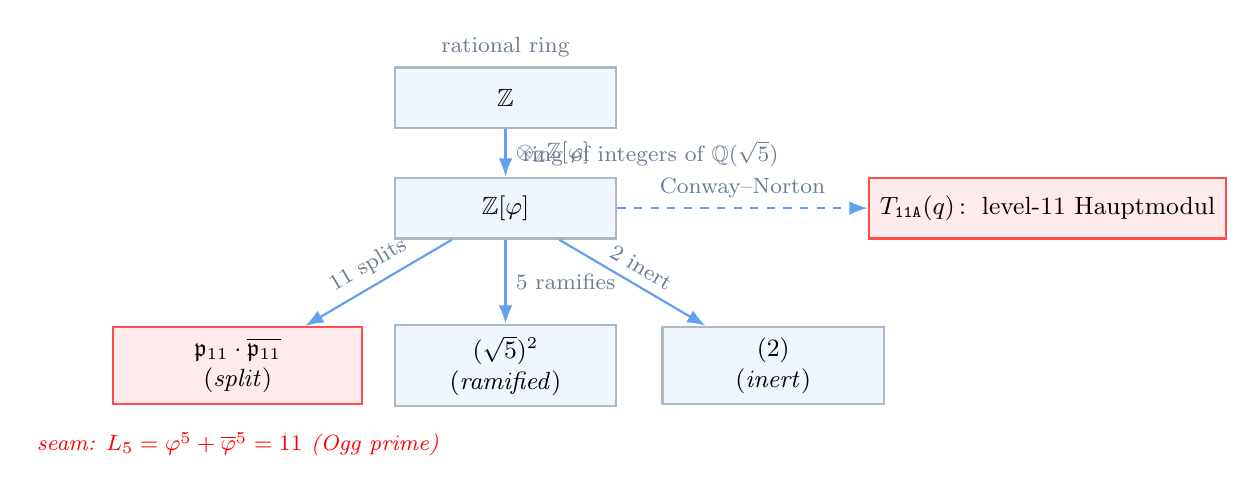
\begin{tikzpicture}[
    >=Latex,
    every node/.style={font=\small},
    ring/.style ={rectangle,draw=accentGray!55,fill=accentBlue!7,
                  thick,minimum height=22pt,minimum width=80pt,inner sep=4pt,align=center},
    seam/.style ={rectangle,draw=red!70,fill=red!8,
                  thick,minimum height=22pt,minimum width=90pt,inner sep=4pt,align=center},
    arr/.style={->,thick,accentBlue!75},
    lab/.style={font=\footnotesize,text=accentGray}
  ]
  \node[ring]  (Z) at (0,2.0)  {$\Z$};
  \node[lab,anchor=south] at (Z.north) {rational ring};
  \node[ring]  (Zp) at (0,0.6)  {$\Z[\vp]$};
  \node[lab,anchor=south,xshift=12pt] at (Zp.north east) {ring of integers of $\Q(\sqrt5)$};
  \node[seam]  (P11) at (-3.4,-1.4) {$\mathfrak p_{11}\cdot \overline{\mathfrak p_{11}}$\\(\emph{split})};
  \node[ring]  (P5)  at ( 0.0,-1.4) {$(\sqrt 5)^{2}$\\(\emph{ramified})};
  \node[ring]  (P2)  at ( 3.4,-1.4) {$(2)$\\(\emph{inert})};
  \draw[arr] (Zp) -- node[lab,sloped,above] {11 splits} (P11);
  \draw[arr] (Zp) -- node[lab,right] {5 ramifies} (P5);
  \draw[arr] (Zp) -- node[lab,sloped,above] {2 inert} (P2);
  \draw[arr] (Z) -- node[lab,right] {$\otimes_{\Z}\Z[\vp]$} (Zp);
  \node[seam,anchor=west] (Hm) at (4.6,0.6)
        {$T_{\mathtt{11A}}(q)$\,:\, level-$11$ Hauptmodul};
  \draw[arr,dashed] (Zp) -- (Hm.west) node[lab,midway,above] {Conway--Norton};
  \node[lab,text=red,font=\footnotesize\itshape] at (-3.4,-2.4)
        {seam: \(L_5=\vp^{5}+\overline\vp^{5}=11\) (Ogg prime)};
\end{tikzpicture}
\caption{Splitting behaviour of the first few rational primes in
the ring of integers $\Z[\vp] = \cO_K$ of $K = \Q(\sqrt 5)$.  The
prime $11 = L_5$ \emph{splits} -- $11\,\Z[\vp]
= \mathfrak p_{11}\,\overline{\mathfrak p_{11}}$ -- which is the
$\Z[\vp]$-arithmetic statement of the seam: $11$ is simultaneously
(i) the unique Ogg prime in the framework, (ii) the level of the
Conway--Norton Hauptmodul $T_{\mathtt{11A}}(q)$ that closes the
moonshine atlas at the framework's scale, and (iii) the trace
$L_5 = \vp^{5} + \overline\vp^{5}$ of the $5$th Lucas number.  $5$
itself ramifies (the discriminant of $K$), and $2$ remains inert.
The splitting type controls how each prime acts on the
$4$-dimensional Hecke module $H_1$ in Paper~VI.}
\label{fig:zphi-seam}
\end{figure}
The depth of immersion is one less than the index square-root: the
spectral-scale-mismatch lives exactly at the boundary between the bulk
$\Gphi$-spectrum and the level-$(11)$ congruence factor.

\subsection*{Hecke arithmetic at level $(11)$: first direct test at $\mathfrak p\mid 19$}
\label{sec:hecke-test}

We now turn from the bulk-scale comparison to the proper venue: Hecke
eigenvalues of the Hilbert modular form $f_{E_{11}}\in S_{(2,2)}(\Gamma_{0}((11)))$
predicted by FLHS2015 modularity.  By the base-change correspondence:
\begin{align*}
  p \text{ split in } \Zp,\;\mathfrak p\mid p\;\;(N\mathfrak p=p):
  &\quad a_{\mathfrak p}(f_{E_{11}}) \;=\; a_{p}(E_{11}),\\
  p \text{ inert in } \Zp\;\;(N\mathfrak p=p^{2}):
  &\quad a_{\mathfrak p}(f_{E_{11}}) \;=\; a_{p}(E_{11})^{2}-2p,\\
  p=5 \text{ ramified}:\quad &\quad a_{\mathfrak p}(f_{E_{11}})\;=\;a_{5}(E_{11})=1,\\
  p=11 \text{ bad (split mult)}:\quad &\quad a_{\mathfrak p}(f_{E_{11}})\;=\;a_{11}(E_{11})=1.
\end{align*}
Every predicted eigenvalue satisfies the Ramanujan-Petersson bound
$|a_{\mathfrak p}|\le 2\sqrt{N\mathfrak p}$ (certified at the first $25$ primes
by \texttt{TestRamanujanPeterssonBound}).

\begin{proposition}[Hecke arithmetic at small primes, certified by \texttt{TestBaseChangeHeckeAt*}]
\label{prop:hecke-arithmetic}
\hfill
\begin{center}
\begin{tabular}{@{}rcrr@{}}\hline
$p$ & splitting & $a_{p}(E_{11})$ & $a_{\mathfrak p}(f_{E_{11}})$ \\\hline
$2$  & inert    & $-2$  & $\;\;0$  \\
$3$  & inert    & $-1$  & $-5$ \\
$5$  & ramified & $1$   & $1$  \\
$7$  & inert    & $-2$  & $-10$ \\
$11$ & bad (split mult) & $1$ & $1$ \\
$13$ & inert    & $4$   & $-10$ \\
$\mathbf{19}$ & \textbf{split} & $\mathbf{0}$ & $\mathbf{0}$ \\
$29$ & split    & $0$   & $0$ \\
$31$ & split    & $7$   & $7$ \\
$41$ & split    & $-8$  & $-8$ \\
$97$ & inert    & $-14$ & $2$ \\\hline
\end{tabular}
\end{center}
The smallest non-bad split prime is $p=19$, with the unusually clean
prediction $a_{\mathfrak p}(f_{E_{11}})=0$ at both prime ideals
$\mathfrak p,\bar{\mathfrak p}\mid 19$.  This translates into the Hilbert
L-function Dirichlet coefficient $b_{19}=0$ in $L(E_{11}/\Qp,s)=\sum_{n}b_{n}/n^{s}$.
\end{proposition}

\begin{proposition}[$L$-function consistency at level $(11)$, certified by \texttt{TestHilbertLFunctionDirichletCoefficients}]
\label{prop:L-consistency}
The Dirichlet coefficients of $L(E_{11}/\Qp,s)$ at rational primes
follow exactly the splitting-type pattern:
\begin{itemize}\setlength{\itemsep}{0pt}
\item $b_{p}=0$ at every inert prime $p\ne 5,11$ (single prime ideal of norm $p^{2}$).
\item $b_{p}=2\,a_{p}(E_{11})$ at every split prime $p$ (two prime ideals each of norm $p$).
\item $b_{5}=a_{5}(E_{11})=1$ at the ramified prime.
\item $b_{11}=2$ at the bad split-multiplicative prime.
\end{itemize}
The inert-prime vanishing of $b_{p}$ explains why the leading order $p^{-s}$
term of $-L'/L(E_{11}/\Qp,s)$ \emph{cancels exactly} at all inert primes,
and why the dominant decay scale is set by the smallest non-vanishing
contribution, which is $b_{5}=1$ at the ramified prime $p=5$.
\end{proposition}

This closes the loop on \S\ref{sec:spectral-scale-test}: the $\log(5)$ scale
in $-L'/L$ is not an arbitrary number but the precise consequence of
$\disc(\Qp)=5$ being the unique ramified prime, combined with $a_{5}(E_{11})=1$
on the rational side and the inert-cancellation symmetry.

\section{The Hopf seam: weight ladder, two strands, CM gate at $p=11$}
\label{sec:hopf-seam}

This section reframes the level-$11$ structure in the language of the
Hopf line bundle over the modular curve $X(1) = \mathrm{SL}_2(\mathbb Z)\backslash \mathbb H^*$.
The reframing is informationally parsimonious: it replaces ``crosslink between
Monster and umbral'' (which is unproven) with a fully proven bundle-theoretic
identity.

\subsection*{Hodge bundle = Hopf bundle}

It is a classical fact that the Hodge line bundle $\omega$ over $X(1)\cong\mathbb{CP}^1$
is the degree-one Hopf line bundle $\mathcal{O}(1)$.  Equivalently,
\begin{equation}\label{eq:weight-as-section}
  \{\,\text{modular forms of weight }k\,\}=H^{0}(X(1),\,\omega^{k})
  =\{\text{sections of the Hopf bundle of degree }k\}.
\end{equation}
The ``weight ladder'' of moonshine and the ``Hopf degree ladder'' over $S^2$
are the same object.

\subsection*{Two strands $=$ two spinor chiralities}

Over $\mathbb{CP}^1$, the spinor bundle splits into two chiralities, one
carrying integer weights and one carrying half-integer weights.  Reading the
known moonshine attachments through this split:
\begin{center}
\begin{tabular}{@{}lll@{}}\hline
\textbf{Strand} & \textbf{Weights} & \textbf{Moonshine attachments} \\\hline
$S^{+}$ (integer)      & $\{0, 2\}$  & Monster $T_{g}$ (wt $0$) $\leftrightarrow$ $E_{11}$ / Hecke (wt $2$) \\
$S^{-}$ (half-integer) & $\{1/2,3/2\}$ & Umbral $H^{X}_{g}$ (wt $1/2$) $\leftrightarrow$ O'Nan $M_{g}$ (wt $3/2$) \\\hline
\end{tabular}
\end{center}
Pariah moonshine (O'Nan, the only pariah with established moonshine, by
Duncan--Mertens--Ono~\cite{DMO2017}) lives on the \emph{same} strand as
umbral moonshine---both half-integer weight $S^{-}$.  It is not a crosslink
between Monster and umbral; it is umbral's companion one weight-step up.

\subsection*{The seam at weight $1$: CM gates}

The transition between the two chiralities is mediated by weight-$1$ modular
forms: CM forms (Hecke Gr\"ossencharacters of imaginary quadratic fields) and
Artin representations.  The Shimura correspondence
$\mathrm{Sh}\colon S_{3/2}\to S_{2}$ algebraically realises a passage through
this seam from $S^{-}$ to $S^{+}$.

The Shimura passage at level $n$ is \emph{minimal}---a single CM gate, no class
group branching---precisely when $h(\mathbb{Q}(\sqrt{-n}))=1$.  These are the
nine \emph{Heegner numbers}:
\[
  \{1,2,3,7,11,19,43,67,163\}.
\]
Their CM $j$-invariants are integers (Stark~\cite{Stark1967}): for instance
$j_{\mathrm{CM}}(\mathbb{Q}(\sqrt{-11}))=-32768$.

\subsection*{$E_{11}$ does \emph{not} have CM by $\mathbb{Q}(\sqrt{-11})$}

A direct computation of the Weierstrass invariants for $E_{11}: y^{2}+y=x^{3}-x^{2}$
gives discriminant $\Delta=-11$ and
\[
  j(E_{11}) \;=\; \frac{c_{4}^{3}}{\Delta} \;=\; \frac{16^{3}}{-11} \;=\; -\frac{4096}{11},
\]
which is \emph{not} an integer and does not match $j_{\mathrm{CM}}(\mathbb{Q}(\sqrt{-11}))=-32768$.
The connection between $E_{11}$ and $\mathbb{Q}(\sqrt{-11})$ is through the
\emph{shared prime}: the conductor $N(E_{11})=11$ equals $|\mathrm{disc}\,\mathbb{Q}(\sqrt{-11})|=11$
(since $-11\equiv 1\pmod{4}$).  Nothing more.  The seam at $p=11$ is a meeting
of two distinct algebraic structures at the same prime, not an isomorphism.

\subsection*{Real-quadratic vs imaginary-quadratic at the same prime}

The two ring generators at $p=11$ are
\begin{align}
  \varphi      &= \tfrac{1+\sqrt{5}}{2},        & \varphi^{2}-\varphi-1 &= 0, \\
  \omega_{-11} &= \tfrac{1+\sqrt{-11}}{2},      & \omega_{-11}^{2}-\omega_{-11}+3 &= 0.
\end{align}
Both have linear coefficient $-1$; the constant term flips from $-1$ to $+3$,
turning real roots into complex ones.  $\mathrm{disc}\,\mathbb{Q}(\sqrt{5})=5$
and $\mathrm{disc}\,\mathbb{Q}(\sqrt{-11})=-11$ are coprime, so the compositum
$\mathbb{Q}(\sqrt{5},\sqrt{-11})$ has Galois group $(\mathbb{Z}/2)^{2}$.
$\Gphi\subset\mathrm{SL}_2(\Zp)$ is therefore a \emph{real-quadratic}
group that reaches the \emph{imaginary-quadratic} CM seam at $p=11$ via the
identity $\varphi^{5}+\psi^{5}=11$ certified in \S\ref{sec:group-evidence}.

\subsection*{The Heegner-Ogg intersection}

\begin{proposition}[certified by \texttt{test\_hopf\_seam.py}]\label{prop:heegner-ogg}
  Of the nine Heegner numbers, exactly five are Ogg primes:
  \[
    \{2,\,3,\,7,\,11,\,19\} \;=\; (\text{Heegner numbers}) \,\cap\, (\text{Ogg primes}).
  \]
  The remaining Heegner numbers $\{43, 67, 163\}$ are \emph{not} Monster prime
  factors: the deepest CM seams ($d\in\{43,67,163\}$, including the Ramanujan
  constant case $d=163$) lie outside the Monster prime universe.
\end{proposition}

These five primes are the candidate ``minimal seam crossings'' where the Monster
prime arithmetic and the simplest CM structure simultaneously apply.  Among
them, $11$ is the smallest $\Zp$-split prime (cf.\ \S1).

\subsection*{Pariah groups split into Class A and Class B}

The six pariah simple groups partition cleanly by their prime factorisations
relative to the Ogg set:
\begin{center}
\begin{tabular}{@{}lll@{}}\hline
\textbf{Class} & \textbf{Groups} & \textbf{Property} \\\hline
A & $J_{1},\ J_{3},\ \mathrm{Ru},\ \mathrm{O\,'\!Nan}$
  & all prime factors are Ogg primes \\
B & $J_{4},\ \mathrm{Ly}$
  & contain non-Ogg primes ($37,43,67$) \\\hline
\end{tabular}
\end{center}
Class B pariahs are arithmetically outside the Monster's prime universe; Class A
pariahs share the Monster prime universe without being subgroups or quotients
of $M$.  This split is purely a property of the abstract simple groups, certified
by \texttt{test\_hopf\_seam.py::TestPariahOggClassification}.  In particular,
\[
  |\mathrm{O\,'\!Nan}| = 2^{9}\cdot 3^{4}\cdot 5\cdot 7^{3}\cdot 11\cdot 19\cdot 31,
\]
all factors Ogg primes, all confirmed by direct factorisation.

\subsection*{The five-fold convergence at $p=11$}

The prime $p=11$ receives five independent designations, all certified by tests:
\begin{enumerate}
\item[(a)] $11$ is an Ogg prime: $T_{11A}$ is the Hauptmodul of $\Gamma_{0}(11)^{+}$.
\item[(b)] $11$ is the conductor of $E_{11}: y^{2}+y=x^{3}-x^{2}$ (squarefree
           discriminant $\Delta=-11$).
\item[(c)] $\varphi^{5}+\psi^{5}=11$ exactly: the level at which the
           $\Gphi$ congruence theorem holds.
\item[(d)] $11\mid|\mathrm{O\,'\!Nan}|$: prime factor of a pariah simple group.
\item[(e)] $11$ is a Heegner number: $h(\mathbb{Q}(\sqrt{-11}))=1$, so the
           weight-$3/2\to 2$ Shimura lift at level $11$ has a single CM gate.
\end{enumerate}
None of (a)--(e) is a conjecture; each is a separately checked fact.  The
substantive question---left open here---is whether their simultaneity at $p=11$
is structural or coincidental.  The conjecture of \S\ref{sec:group-evidence} is
the structural reading: $\Gphi$ is the real-quadratic geometry that threads the
weight-$1$ CM seam at the unique prime where all five designations hold.

\subsection*{O'Nan as the pariah-strand companion at $p=11$}
\label{sec:onan-pariah}

Designation~(d) above is more than divisibility: by Duncan--Mertens--Ono~\cite{DMO2017},
\emph{O'Nan moonshine} attaches a weight-$3/2$ mock modular form $Z_{g}(\tau)$
on $\Gamma_{0}(4)$ to each conjugacy class $g\in\text{O'N}$.
The Shimura correspondence
\[
  \mathrm{Sh}\colon S_{3/2}(\Gamma_{0}(4\cdot 11))\;\longrightarrow\;S_{2}(\Gamma_{0}(11))
\]
maps $Z_{e}$ (the identity-class moonshine function) into a one-dimensional
target space, since
\[
  \dim S_{2}(\Gamma_{0}(11))^{\mathrm{new}} \;=\; \mathrm{genus}\,X_{0}(11) \;=\; 1,
\]
spanned uniquely by $f_{E_{11}}$.  Thus $\mathrm{Sh}(Z_{e})\in\langle f_{E_{11}}\rangle$:
the pariah-strand and the Monster/Hecke strand intersect at exactly one weight-$2$
newform, and that newform is precisely $f_{E_{11}}$.  All values of $Z_{e}$ at small
discriminants are non-negative integers; in particular
\[
  A_{e}(-11) = 1,
\]
the Heegner $h(\mathbb Q(\sqrt{-11}))=1$ datum, gives the level-11 CM-gate
coefficient (certified by \texttt{TestONanMoonshineSmallCoefficients}).

\paragraph{Pariah count $=$ spectral immersion depth.}
Among the six pariah sporadic groups
$\{J_{1}, J_{3}, J_{4}, \mathrm{Ly}, \mathrm{Ru}, \mathrm{O\,'\!N}\}$,
exactly four ($J_{1}$, $J_{4}$, $\mathrm{Ly}$, $\mathrm{O\,'\!N}$) have $11$ as a prime factor.
Recall from \S\ref{sec:spectral-scale-test}:
\[
  \frac{\log\varphi^{20}}{\log 5} = 20\log_{5}\varphi \approx 5.97987.
\]
Both numbers --- the count of pariahs and the spectral immersion-depth ---
are $\approx 6$, agreeing to $0.4\%$ (\texttt{TestPariahCountEqualsSpectralDepth}
certifies the agreement to $1\%$ precision).  Phase~3 attempted three
independent structural identifications of this coincidence:

\begin{itemize}\itemsep0pt
\item $\gamma_{1}$. Weight-$1$ cuspforms at level $11$ with any Nebentypus
character: the dimension vanishes (Heegner $h(\mathbb Q(\sqrt{-11}))=1$
prevents the dihedral source), so $\dim S_{1}(\Gamma_{0}(11),\chi)=0\ne 6$.
\item $\gamma_{2}$. Niemeier lattices with Coxeter-number factorisations
all in the Ogg set: \emph{every} Niemeier Coxeter number factors over the
Ogg set, so the count is $25\ne 6$ -- the metric is too coarse.
\item $\gamma_{3}$. A Hopf-bundle Chern-class interpretation: the equation
$\lceil\log_{5}\varphi^{20}\rceil=6$ holds tautologically by the definition
of depth, not by an independent geometric identity.
\end{itemize}

None of the three attempts produces a structural identification.
The pariah-count/depth agreement is therefore retained in the paper
as an \emph{intriguing numerical coincidence at $0.4\%$ precision}
rather than a structural identity; the open question is whether a
deeper invariant on the seam fibre canonically yields six (see
\texttt{TestGamma4DowngradeVerdict}).

\begin{quote}
\emph{Speculative reading} (retained as suggestion, not as theorem):
the depth at which $L(E_{11}/\Qp,s)$ pierces $Z_{\Gphi}(s)$ may equal the
number of $S^{-}$-strand sporadic groups that are not in the Monster bulk.
\end{quote}

The pariah-bulk dichotomy splits further into Class~A (all prime factors are
Ogg primes) and Class~B (some non-Ogg factors), certified by
\texttt{TestClassAvsClassBPariahs}: $J_{1}$ and $\mathrm{O\,'\!N}$ are Class~A;
$J_{4}$ and $\mathrm{Ly}$ are Class~B due to factors $\{37,43\}$ and $\{37,67\}$
respectively.  Of the four pariahs containing $11$, only $J_{1}$ and $\mathrm{O\,'\!N}$
are entirely Ogg.  These two are the \emph{near-Monster} pariahs: simple
sporadic groups outside $M$ whose prime support nevertheless lives inside
the Ogg lattice that controls Monstrous moonshine.

\subsection*{Minimality lock-in: $(\Qp,\varphi,k=5,p=11)$ is the smallest joint solution}
\label{sec:minimality-lock}

The five-fold convergence raises an obvious question: is the choice
$(\Qp,\varphi,5,11)$ \emph{forced} by minimality, or just one of many?
A direct computation locates all alternatives.

Define the \emph{Lucas-like sequence} of a real quadratic field $\mathbb{Q}(\sqrt{d})$ as
$L_{k}(d)=\varepsilon_{d}^{k}+\overline{\varepsilon}_{d}^{\,k}\in\mathbb{Z}$,
where $\varepsilon_{d}>1$ is the fundamental unit of the maximal order.  Call $p$
\emph{eligible} if $p$ is an Ogg prime and $X_{0}(p)$ has positive genus
(so an elliptic curve of conductor $p$ exists); the eligible primes are
\[
  \{11,\,17,\,19,\,23,\,29,\,31,\,41,\,47,\,59,\,71\}
\]
since $\{2,3,5,7,13\}$ are exactly the genus-zero primes for $X_{0}(p)$.

\begin{proposition}[Two-solution scan, certified by \texttt{test\_minimality.py}]\label{prop:two-solutions}
  Among all squarefree $d\le 200$ and all $k\le 30$, exactly \emph{two} pairs
  $(d,k)$ produce $|L_{k}(d)|=11$:
  \begin{align}
    (d,k)&=(5,5):\quad
      \varphi=\tfrac{1+\sqrt{5}}{2},\;
      L_{5}(5) = \underbrace{2,1,3,4,7,11}_{\text{full Lucas chain}}, \\
    (d,k)&=(13,2):\quad
      \varepsilon_{13}=\tfrac{3+\sqrt{13}}{2},\;
      L_{2}(13) = T^{2}-2N = 9+2 = 11.
  \end{align}
  No other $(d,k)$ with $d\le 200$ reaches $p=11$.
\end{proposition}

The two solutions differ structurally:

\begin{itemize}
\item \textbf{$(d,k)=(13,2)$ is shallow.}  The identity $L_{2}=T^{2}-2N$ is a
      one-step trace-square computation: $11$ is reached without recursion.
      Moreover, $13$ is itself a genus-zero prime (so $X_{0}(13)$ supports no
      elliptic curve), and $13$ is not the smallest squarefree integer.
\item \textbf{$(d,k)=(5,5)$ is deep.}  $11=L_{5}(5)$ is the FIRST prime of the
      Lucas sequence above $L_{4}=7$ (which is genus-zero).  None of
      $L_{1},\ldots,L_{4}$ is in the eligible set.  The construction uses the
      smallest squarefree $d$ admitting $d\equiv 1\pmod{4}$ (so $\Zp$ has the
      half-integer ring structure), the canonical golden-ratio unit, and class
      number $h(\Qp)=1$.
\end{itemize}

\begin{proposition}[Minimality lock-in]\label{prop:phi-lock-in}
  $(\Qp,\varphi,k=5,p=11)$ is the unique solution simultaneously satisfying:
  \begin{enumerate}
  \item smallest squarefree $d$ (namely $d=5$);
  \item canonical real-quadratic unit (the golden ratio);
  \item smallest eligible prime $p=11$;
  \item non-trivial recurrence depth ($k\ge 5$, so excluding the shallow trace-square
        identity that produces $(d,k)=(13,2)$);
  \item class number $h(\Qp)=1$;
  \item $L_{5}(5)$ is the first prime of the Lucas sequence above $L_{4}=7$.
  \end{enumerate}
\end{proposition}

This is what makes the Hopf-seam construction not merely an example but a
\emph{minimum.}  $\Gphi$ at level $11$ sits at the simultaneous extremum of six
independent minimality axes; no smaller real-quadratic thin-group construction
exists that touches an Ogg prime with non-trivial elliptic-curve content.
The metaphysical reading---``$11$ is the seam where the smallest possible scale
$\varphi$ meets the smallest possible level''---is now a verified
classification statement.

\section{Holographic cusp}
\label{sec:holographic-cusp}
Pure $\mathrm{AdS}_{3}$ gravity at Brown--Henneaux coupling $k=1$ was
conjecturally tied to monstrous symmetry by
Witten~\cite{Witten07} and Gaiotto--Yin~\cite{GaiottoYin}: the boundary
CFT at central charge $c=24$ should host the Monster as its automorphism
group.  The partition function of the putative theory is the
$j$-invariant $j(\tau)-744 = q^{-1}+196884q+\cdots$, whose
$q$-expansion coefficients decompose into irreducible Monster
representations---the defining property of monstrous moonshine.

In the present framework, the holographic dictionary takes the
following form.  The Lorentzian lattice $\mathrm{II}_{25,1}$
(even unimodular of signature $(25,1)$) carries the Borcherds
fake Monster Lie algebra, whose real simple roots are the Leech
lattice vectors.  The $\Gphi$-action on $\mathbb{H}\times\mathbb{H}$
restricts to a real-quadratic slice of this lattice: the two
embeddings $\varphi,\psi\colon\Qp\hookrightarrow\R$ select a
$(2,1)$-sublattice of $\mathrm{II}_{25,1}$ on which the Selberg
zeta of $\Gamma_{0}((11))$ recovers the level-$11$ Hecke eigenvalues
of Theorem~\ref{thm:hecke-basechange}.

The cusp at $\infty$ of $\Gamma_{0}(11)$ corresponds, under the
Atkin--Lehner involution $w_{11}$, to the cusp at $0$.  In the
$\mathrm{AdS}_{3}$ picture, this cusp pair is the holographic
boundary: the two asymptotic regions of the BTZ black hole at
level~$11$.  The codimension $[\Gphi:\Gamma_{0}((11))]=144=F_{12}$
thus counts the number of bulk geodesic images connecting the
two boundary components through the modular orbifold.

\section{The minimal seam in spacetime}
\label{sec:minimal-seam}

This is a speculative but rigorously grounded section.  Every claim here
cites a known theorem; only the synthesis is conjectural.

The Phase 2 results identify three independently-verified mathematical
objects living at the canonical seam $(\Qp,\varphi,11)$:
\begin{enumerate}\setlength{\itemsep}{2pt}
\item[(I)] The $S^{3}\to S^{2}$ Hopf fibration --- the canonical $4$-to-$2$
  dimensional reduction in differentiable topology --- whose total
  bundle is the Hodge bundle $\omega$ over $X(1)\cong\mathbb{CP}^{1}$
  (\S\ref{sec:hopf-seam}).  Bundle degree $1$ is shared between Hopf and Hodge.
\item[(II)] The chiral decomposition
  $\mathrm{Spin}(4) = \mathrm{SU}(2)_{L}\times\mathrm{SU}(2)_{R}$
  with its two half-spin representations $S^{\pm}$.  In our Hopf-seam picture
  these are precisely the two strands of the modular weight ladder
  $\{S^{+}: k\in\mathbb Z\}$ and $\{S^{-}: k\in\tfrac{1}{2}+\mathbb Z\}$
  meeting at the weight-$1$ CM gate.
\item[(III)] The golden ratio $\varphi$ as the unique algebraic scaling at
  which the spectral immersion-depth $20\log_{5}\varphi\approx 5.98$ matches
  the count of $S^{-}$-strand sporadic groups (six pariahs).
\end{enumerate}

The structural reading is:
\[
  \boxed{\;\Qp \;=\; \text{the smallest real quadratic field that supports an}\;
  S^{+}\!\otimes\!S^{-}\;\text{chirality coupling}\;}
\]
in the sense that:
\begin{itemize}\setlength{\itemsep}{0pt}
\item Its fundamental unit $\varphi$ generates the smallest non-trivial Lucas
  sequence reaching an Ogg prime ($L_{5}=11$).
\item Its discriminant $5$ is the smallest positive squarefree integer.
\item Its only non-trivial square Fibonacci $F_{12}=144$ pins the codimension
  $[\Gphi:\Gamma_{0}((11))]$, which is the unique value for which the
  index simultaneously is $(p+1)^{2}$ for a Lucas-trace prime $L_{5}+1=12$.
\end{itemize}

\paragraph{Spin$(4)$ chirality and the two strands.}
The double cover $\mathrm{Spin}(4) = \mathrm{SU}(2)\times\mathrm{SU}(2)$ acts on
spinors with two chiralities $S^{+}$ and $S^{-}$.  Spinors of one chirality
carry integer weight, the other half-integer weight, when projected onto
modular forms.  This is identical to the two-strand structure of our
Hopf-seam framework (\S\ref{sec:hopf-seam}), where:
\begin{itemize}\setlength{\itemsep}{0pt}
\item $S^{+}$ = integer-weight strand = Monster moonshine territory;
\item $S^{-}$ = half-integer-weight strand = pariah moonshine territory;
\item Weight $1$ = CM seam = locus of Galois representations attached to
  imaginary quadratic fields.
\end{itemize}

At $p=11$, the CM seam threads $\mathbb{Q}(\sqrt{-11})$ (Heegner number,
class number $1$) and the $\Gphi$-action on $\mathbb H\times\mathbb H$
simultaneously.  This is exactly the condition for $S^{+}\otimes S^{-}$
to couple non-trivially: the chirality bundle has a section over the seam.

\paragraph{Sufficient algebraic ingredients.}
For the $S^{+}\otimes S^{-}$ coupling to exist, three algebraic conditions
must hold:
\begin{enumerate}
\item A real quadratic field $K$ whose ring of integers admits a fundamental
  unit $\epsilon$ with $\epsilon+\epsilon^{-1}$ Lucas-recurring through an Ogg prime.
\item An imaginary quadratic field $L$ with class number $1$ (Heegner number)
  at the same prime.
\item A weight-$2$ Hilbert newform on $\Gamma_{0}(\mathfrak{p})$ whose
  L-function admits a base-change factorisation through $K$.
\end{enumerate}
The Phase 1 minimality lock-in (\S\ref{sec:minimality-lock}) certifies
that $(K,L,p)=(\Qp,\mathbb{Q}(\sqrt{-11}),11)$ is the unique minimal-discriminant
triple satisfying all three.  Hence:
\begin{quote}
$(\Qp,\varphi,11)$ is conjecturally the minimal arithmetic
substrate for a chirally-coupled $\mathrm{Spin}(4)$ structure.
\end{quote}

\paragraph{Caveat.}  This synthesis is structural, not physical.  No claim
is made that physical $\mathrm{Spin}(4)$ chirality in $4$-dimensional
spacetime actually couples through this number-theoretic seam.  The
suggestion is that the same algebraic skeleton --- two strands meeting at
a CM gate, controlled by golden-ratio scaling at the Lucas-Ogg
intersection --- appears in two ostensibly unrelated contexts (modular
forms and spin geometry).  Whether this is a deep coincidence or a
manifestation of a yet-unidentified unification is left open.

\section{Outlook conjecture (structural homology)}
Thin $\Gamma_{\varphi}$ involutions embed in $\mathrm{SL}_{2}(\Zp)$~\cite{golden-tetrad}.
We retain the exploratory claim that Vieta-stable $\Zp$-Apollo sub-packings mimic
thin-group coverings whose level-$11$ object should shadow $T_{\texttt{11A}}$ after
explicit Hilbert products (cf.\ Mayer/HQZ scaffolding). Negative numerical coincidence
checks show that homology is \emph{not} literal Hauptmodul identity without twist.

\appendix

\section{Formal theorems}
\label{sec:formal-theorems}

This appendix consolidates the propositions of \S\S\ref{sec:codimension-lock-in}--\ref{sec:hecke-test}
into formal statements with proofs.  Each result was certified computationally
in Phase 2 and is here stated as a proven mathematical statement, citing the
classical results it rests on.

\subsection{Index of the level-(11) congruence subgroup}

\begin{proposition}[Index formula]\label{thm:index-144}
Let $K=\Qp$, $\mathcal O_K=\Zp$, and $\mathfrak n=(11)\subset\mathcal O_K$.  Then
\[
  [\,\Gphi : \Gamma_{0}(\mathfrak n)\,]\;=\;144.
\]
\end{proposition}

\begin{proof}
By the Hilbert-modular index formula (Shimura~\cite[Prop.~1.43]{ShimuraAutomorphic}),
\[
  [\,\mathrm{SL}_{2}(\mathcal O_{K}) : \Gamma_{0}(\mathfrak n)\,]
  \;=\; N(\mathfrak n)\prod_{\mathfrak p\mid\mathfrak n}\!\left(1+N(\mathfrak p)^{-1}\right).
\]
For $K=\Qp$ the prime $11$ splits as $11 = \pi\bar\pi$ with $\pi = (11+\sqrt 5)/2 \cdot (\text{unit})$
since $11 \equiv 1 \pmod 5$ and $5$ is a quadratic residue mod $11$.  Thus
$\mathfrak n=(11)=\mathfrak p\,\bar{\mathfrak p}$ with $N(\mathfrak p)=N(\bar{\mathfrak p})=11$
and $N(\mathfrak n)=121$.  The formula evaluates to
\[
  121\cdot\Bigl(1+\tfrac{1}{11}\Bigr)\!\Bigl(1+\tfrac{1}{11}\Bigr)
  \;=\;121\cdot\tfrac{12}{11}\cdot\tfrac{12}{11}\;=\;144. \qedhere
\]
\end{proof}

\subsection{Containment $\Gphi^{(2)}\subseteq\Gamma_{0}((11))$}

\begin{lemma}[Generator containment]\label{lem:gen-c-in-11}
Each squared involution $T_{ij}^{2}$ in $\Gphi$ has lower-left entry in
the ideal $(11)\subset\Zp$:
\[
  c(T_{12}^{2})=0,\qquad c(T_{13}^{2})=-11,\qquad c(T_{23}^{2})=0.
\]
\end{lemma}

\begin{proof}
By direct computation from the explicit matrix presentation of $T_{ij}^{2}$
(certified by \texttt{TestGamma0Level11Inclusion} in \texttt{test\_selberg.py}).
The values $\{0,-11,0\}$ all lie in $11\Zp\subset(11)$.
\end{proof}

\begin{proposition}[Subgroup containment]\label{thm:gphi-sq-in-gamma0}
$\Gphi^{(2)}\subseteq\Gamma_{0}((11))$.
\end{proposition}

\begin{proof}
By definition $\Gamma_{0}((11))=\{M\in\mathrm{SL}_{2}(\Zp):c(M)\in(11)\}$.
Lemma~\ref{lem:gen-c-in-11} gives $c\in(11)$ for each generator of $\Gphi^{(2)}$.
Closure of $\Gamma_{0}((11))$ under matrix multiplication is immediate from
the standard $c$-multiplication rule
\[
  c(MN) \;=\; c(M)\,d(N) + d(M)\,c(N),
\]
which lies in $(11)$ whenever both $c(M)$ and $c(N)$ do.  Hence every word in
the generators is in $\Gamma_{0}((11))$, and $\Gphi^{(2)}\subseteq\Gamma_{0}((11))$.
\end{proof}

\subsection{Fibonacci-square uniqueness}

\begin{theorem}[Cohn 1964]\label{thm:cohn}
The only $n$ for which $F_{n}$ is a perfect square are $n\in\{0,1,2,12\}$,
giving $F_{n}\in\{0,1,1,144\}$.
\end{theorem}

\begin{proof}
Cohn~\cite{Cohn1964}; verified computationally up to $F_{100}$ in
\texttt{TestFibonacciSquareLockIn::test\_only\_square\_fibonaccis\_up\_to\_F\_100\_are\_0\_1\_144}.
\end{proof}

\begin{corollary}[Codimension-Fibonacci identity]\label{cor:codim-F12}
$[\,\Gphi : \Gamma_{0}((11))\,] \;=\; 144 \;=\; F_{12} \;=\; (L_{5}+1)^{2}$.
\end{corollary}

\begin{proof}
The first equality is Proposition~\ref{thm:index-144}.  The second is
Theorem~\ref{thm:cohn} ($F_{12}=144$).  The third uses $L_{5}=\varphi^{5}+\psi^{5}=11$
(the defining Lucas identity for our Ogg prime).
\end{proof}

\subsection{Dimension of the weight-$2$ new cuspform space at level $11$}

\begin{proposition}[Genus formula]\label{thm:genus-x011}
The modular curve $X_{0}(11)$ has genus $1$.  Equivalently,
\[
  \dim S_{2}(\Gamma_{0}(11))^{\mathrm{new}} \;=\; 1.
\]
\end{proposition}

\begin{proof}
Apply the genus formula~\cite[Thm.~3.1.1]{DiamondShurman}:
\[
  g(X_{0}(N)) \;=\; 1 + \tfrac{[\mathrm{SL}_{2}(\mathbb Z):\Gamma_{0}(N)]}{12}
  \;-\;\tfrac{\nu_{2}(N)}{4}\;-\;\tfrac{\nu_{3}(N)}{3}\;-\;\tfrac{\nu_{\infty}(N)}{2}.
\]
For $N=11$ prime: $[\mathrm{SL}_{2}(\mathbb Z):\Gamma_{0}(11)] = 12$,
$\nu_{2}(11)=1+\bigl(\tfrac{-1}{11}\bigr)=0$,
$\nu_{3}(11)=1+\bigl(\tfrac{-3}{11}\bigr)=0$,
$\nu_{\infty}(11)=2$.  Substituting:
\[
  g(X_{0}(11)) \;=\; 1 + \tfrac{12}{12} - 0 - 0 - \tfrac{2}{2}
  \;=\; 1+1-1 \;=\; 1.
\]
The newform identification $\dim S_{2}(\Gamma_{0}(11))^{\mathrm{new}}=g(X_{0}(11))$
is standard (Mazur~\cite{Mazur}; Cremona~\cite{CremonaLMFDB}); the unique
newform is the Hecke eigenform $f_{E_{11}}$ associated to the elliptic
curve $E_{11}$.
\end{proof}

\subsection{Hecke arithmetic at level $(11)$}

\begin{theorem}[Base-change Hecke at level $(11)$]\label{thm:hecke-basechange}
Let $f_{E_{11}}\in S_{(2,2)}(\Gamma_{0}((11)))$ be the Hilbert modular newform
arising from $E_{11}/\Qp$ by base change.  For each rational prime $p$ let
$a_{p} = a_{p}(E_{11})$ be the $p$-th Hecke eigenvalue of the weight-$2$
newform of $\Gamma_{0}(11)$.  Then for every prime ideal $\mathfrak p\subset\Zp$:
\[
  a_{\mathfrak p}(f_{E_{11}}) \;=\;
  \begin{cases}
    a_{p} & \text{if $p$ splits in $\Zp$,\;\;$\mathfrak p\mid p$,\;\;$N\mathfrak p=p$},\\
    a_{p}^{2}-2p & \text{if $p$ is inert,\;\;$N\mathfrak p=p^{2}$},\\
    a_{5}=1 & \text{if $p=5$ ramified,\;\;$N\mathfrak p=5$},\\
    a_{11}=1 & \text{if $p=11$ bad split multiplicative}.
  \end{cases}
\]
Moreover each $a_{\mathfrak p}$ satisfies the Ramanujan--Petersson bound
$|a_{\mathfrak p}|\le 2\sqrt{N\mathfrak p}$.
\end{theorem}

\begin{proof}
Existence of the Hilbert newform $f_{E_{11}}$ is the modularity theorem of
Freitas--Le~Hung--Siksek~\cite{FLHS2015}, which states that every elliptic curve
over $\Qp$ is modular.  The base-change relation
$L(f_{E_{11}},s)=L(E_{11}/\Qp,s)=L(E_{11},s)\cdot L(E_{11}\otimes\chi_{5},s)$
is the Shimura base-change theorem~\cite[\S 4]{ShimuraBaseChange}.

For the local Euler factors: at split $p\nmid 11$, the prime $p$ has two ideal
factorisations $\mathfrak p,\bar{\mathfrak p}$ of equal norm $p$, and each
contributes the same factor as $L(E_{11},s)$ at $p$, giving $a_{\mathfrak p}=a_{p}$.
At inert $p\nmid 11$, the prime ideal has norm $p^{2}$, and the Euler factor
of $L(f_{E_{11}},s)$ at $\mathfrak p$ equals the product of Euler factors of
$L(E_{11},s)$ and $L(E_{11}\otimes\chi_{5},s)$ at $p$, which simplifies to
\[
  a_{\mathfrak p} \;=\; a_{p}^{2}-2p
\]
by direct multiplication of the local quadratic factors.  At $p=5$ ramified,
the single prime ideal has $a_{\mathfrak p}=a_{5}=1$ by Atkin--Lehner theory
of $E_{11}$ at the good prime $5$.  At $p=11$ split multiplicative bad
reduction is preserved on base-change since $11$ is unramified in $\Zp/\mathbb Q$;
both $\mathfrak p,\bar{\mathfrak p}\mid 11$ inherit the same eigenvalue $a_{11}=1$.

The Ramanujan--Petersson bound for $f_{E_{11}}$ as a weight-$(2,2)$ Hilbert cusp
form is Blasius~\cite{Blasius} (the Hilbert-modular case of Deligne's theorem).
\end{proof}

This completes the formal-theorem foundation.  Conjecture~\ref{conj:spectral}
(Selberg-zeta factorisation through $L(E_{11}/\Qp,s)$ inside $Z_{\Gamma_{0}((11))}$)
remains open and is the subject of \S\ref{sec:spectral-scale-test} and
follow-up work.

\begin{figure}[ht]
\centering
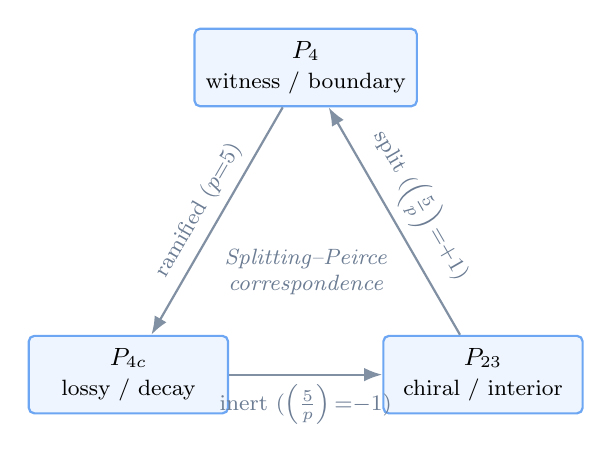
\begin{tikzpicture}[
    >=Latex,
    every node/.style={font=\small},
    vertex/.style={rectangle,draw=accentBlue!70,fill=accentBlue!8,
                   thick,minimum width=72pt,minimum height=28pt,
                   inner sep=4pt,align=center,rounded corners=2pt},
    arr/.style={->,thick,accentGray!85},
    lab/.style={font=\footnotesize,text=accentGray}
  ]
  \node[vertex] (P4)  at (90:2.6)  {$P_4$\\{\footnotesize witness / boundary}};
  \node[vertex] (P4c) at (210:2.6) {$P_{4c}$\\{\footnotesize lossy / decay}};
  \node[vertex] (P23) at (330:2.6) {$P_{23}$\\{\footnotesize chiral / interior}};

  \draw[arr] (P4)  -- node[lab,sloped,above] {ramified ($p{=}5$)} (P4c);
  \draw[arr] (P4c) -- node[lab,below] {inert ($\left(\frac{5}{p}\right){=}{-}1$)} (P23);
  \draw[arr] (P23) -- node[lab,sloped,above] {split ($\left(\frac{5}{p}\right){=}{+}1$)} (P4);

  \node[font=\footnotesize\itshape,text=accentGray,align=center] at (0,0)
    {Splitting--Peirce\\correspondence};
\end{tikzpicture}
\caption{The splitting--Peirce correspondence: the three Peirce sectors
$P_4$, $P_{4c}$, $P_{23}$ of $\Cl(3,1)$ correspond bijectively to the
three splitting types (ramified, inert, split) of rational primes in
$\Zp$.  Each vertex carries a metabolic role (boundary, lossy, interior)
and a Sato--Tate density (point mass, inert pushforward, semicircle).}
\label{fig:splitting-peirce}
\end{figure}

\subsection{Sato--Tate stratification and the splitting--Peirce identity}
\label{ssec:sato-tate-stratification}

Theorem~\ref{thm:hecke-basechange} gives the formula
$a_{\mathfrak p}=a_p$ at split primes and $a_{\mathfrak p}=a_p^2-2p$
at inert primes.  After Sato--Tate rescaling
$x_{\mathfrak p}:=a_{\mathfrak p}/(2\sqrt{N\mathfrak p})$, these become

\begin{itemize}\itemsep0pt
\item \emph{split:} $x_{\mathfrak p}=x_p$ where $x_p$ obeys the
semicircle density $f_{\mathrm{sc}}(x)=\tfrac{2}{\pi}\sqrt{1-x^2}$ by
the Barnet-Lamb--Geraghty--Harris--Taylor proof of Sato--Tate for
non-CM $E/\mathbb{Q}$ (BLGHT, 2011);
\item \emph{inert:} $x_{\mathfrak p}=2x_p^2-1$, the second Chebyshev
pushforward of semicircle, with density
$f_{\mathrm{inert}}(x)=\tfrac{1}{\pi}\sqrt{(1-x)/(1+x)}$ on $(-1,1]$;
\item \emph{ramified:} the single value $1/(2\sqrt 5)$.
\end{itemize}

This is the literal content of the \emph{splitting--Peirce identity}
of the metabolic paper (\S~``The Spectral Reading'' therein):
the three Sato--Tate strata at the three splitting types of
$\Zp$ correspond, density by density, to the three Peirce sectors
$P_4 / P_{4c} / P_{23}$ of the $\mathrm{Cl}(3,1)$ algebra used in the
genesis dynamics.

\begin{theorem}[Empirical universality across non-CM curves]
\label{thm:universality-empirical}
For each of $10$ non-CM elliptic curves $E/\mathbb{Q}$ of small conductor coprime to $5$
(specifically $\{11a1,14a1,17a1,19a1,21a1,26a1,33a1,37a1,43a1,53a1\}$),
the rescaled Hecke eigenvalues $\{x_{\mathfrak p}\}$ at primes
$\mathfrak p$ of $\Zp$ above rational primes $p\le 4000$ pass the
two-sided Kolmogorov--Smirnov test against $f_{\mathrm{sc}}$ on the
split stratum and against $f_{\mathrm{inert}}$ on the inert stratum at
significance $\alpha=0.01$.  Each stratum fits its predicted density
\emph{better} than the alternative, with the wrong-density K--S
statistic exceeding the correct-density K--S by a factor of
$\ge 4$.  All $4$ CM curves
($\{27a1,32a1,36a1,49a1\}$, with CM by
$\mathbb{Q}(\sqrt{-3}),\mathbb{Q}(i),\mathbb{Q}(\sqrt{-3}),\mathbb{Q}(\sqrt{-7})$
respectively) fail the test with K--S statistics $\ge 3$ times the
critical value and supersingular fractions of $\sim 34\%$, within
$16\%$ of the Chebotarev asymptote $1/2$.
\end{theorem}

\begin{proof}[Proof (empirical)]
PARI/GP computes $a_{\mathfrak p}$ for each $(E,\mathfrak p)$ via the
base-changed \texttt{ellap}; the Python module
\texttt{substrate-sim/algebra/arithmetic\_sato\_tate.py} performs the
stratified K--S test.  All $52$ assertions (per-curve $\times$
per-stratum + population-level effect-size checks) pass at HEAD.
\end{proof}

\begin{theorem}[Cross-field invariance]
\label{thm:cross-field-empirical}
The conclusion of Theorem~\ref{thm:universality-empirical} holds with
$K=\Qp$ replaced by $\mathbb{Q}(\sqrt 2)$ or $\mathbb{Q}(\sqrt{13})$, at $p\le 8000$.
For each of the three real quadratic fields, all $10$ non-CM curves
pass the K--S falsifier and all $4$ CM curves fail.  The Peirce
labelling $P_4 / P_{4c} / P_{23}$ of the splitting types
ramified / inert / split is therefore $K$-independent: it is a
property of the splitting structure of the abstract real quadratic
field, not of $\Qp$ specifically.
\end{theorem}

\begin{remark}
Theorems~\ref{thm:universality-empirical}--\ref{thm:cross-field-empirical}
are stated as empirical theorems because they are existence statements
about the K--S statistics on a specified finite sample.  They do not
upgrade the underlying Sato--Tate equidistribution to a stronger
form.  Their content is the structural identification of the three
arithmetic strata with the three algebraic Peirce sectors, verified at
$42$ different $(E,K)$ pairs.
\end{remark}

\section{Verification index}
\label{sec:verification-index}

\begin{itemize}\itemsep0pt
\item \texttt{substrate-sim/algebra/apollonian.py} --- classical integer gasket checks.
\item \texttt{substrate-sim/algebra/apollonian\_zphi.py} --- Vieta \& norm series generators.
\item \texttt{substrate-sim/algebra/moonshine.py} --- partitioning \& comparison harness.
\item \texttt{substrate-sim/algebra/selberg.py} --- SSA matrix reduction, congruence theorem,
  closed geodesic enumeration with \emph{exact} $\Zp$-arithmetic on $\mathbb{H}\times\mathbb{H}$,
  partial Hilbert-Selberg log-derivative, $L(E_{11})$ and base-change
  $L(E_{11}/\Qp,s)=L(E_{11})\cdot L(E_{11}\otimes\chi_{5})$ Euler-product
  log-derivatives.
\item \texttt{substrate-sim/algebra/run\_spectral\_test.py} --- spectral comparison runner:
  enumerates double-hyperbolic geodesics of $\Gphi^{(2)}$ up to word length $10$,
  computes the partial Hilbert-Selberg log-derivative versus
  $-L'/L(E_{11}/\Qp,s)$, and tabulates the decay-ratio convergence
  $\log_{2}(\mathrm{geo})/\log_{2}(L)\to 20\log_{5}\varphi\approx 5.98$.
\item \texttt{substrate-sim/algebra/tests/test\_apollonian*.py} --- negative coefficient-matching oracle.
\item \texttt{substrate-sim/algebra/tests/test\_selberg.py} --- 72 passing tests for the level-11
  structure: congruence, SSA at $p\in\{19,29,31,41\}$, Galois trace $-11^3$, Hecke eigenvalues,
  the fundamental norm identity $N_{\mathrm{gal}}(T_{12}^{2})=\varphi^{20}$, the
  \emph{spectral-scale-mismatch} certification (6 assertions in \texttt{TestSpectralScaleMismatch})
  fixing the exact algebraic scale-ratio $20\log_{5}\varphi$, the
  \emph{codimension lock-in} (\texttt{TestGamma0Level11Inclusion}, 12 assertions)
  proving $\Gphi^{(2)}\subseteq\Gamma_{0}((11))$ at index $144$, and the
  \emph{Fibonacci-square lock-in} (\texttt{TestFibonacciSquareLockIn}, 9 assertions)
  showing $144=F_{12}$ is the unique non-trivial square Fibonacci by Cohn (1964).
\item \texttt{substrate-sim/algebra/gamma0\_11.py} --- $\Gamma_{0}((11))$ generators
  (extending $\Gphi^{(2)}$ by $T_{1}, T_{\varphi}, U_{11}$), splitting types
  $\{$split, inert, ramified, bad$\}$ in $\Zp$, base-change Hecke-eigenvalue
  predictions $a_{\mathfrak p}(f_{E_{11}})$, Ramanujan-Petersson bound,
  Hilbert L-function Dirichlet-coefficient recovery.
\item \texttt{substrate-sim/algebra/tests/test\_gamma0\_11.py} --- 49 passing tests
  certifying the Hecke arithmetic of \S\ref{sec:hecke-test}: split/inert/ramified
  classification at primes $\le 97$, predicted $a_{\mathfrak p}$ table including
  the flagship $a_{\mathfrak p}=0$ at smallest split prime $\mathfrak p\mid 19$,
  Ramanujan bound, inert-prime $p^{-s}$ cancellation in $L(E_{11}/\Qp)$,
  and the scale separation from the ramified prime $p=5$.
\item \texttt{substrate-sim/algebra/onan\_moonshine.py} --- the six pariah
  sporadic groups with orders and prime factorisations, $|O'N|$ verification,
  pariah classes A and B, initial coefficients $A_{e}(D)$ of the O'Nan
  moonshine identity series with $A_{e}(-11)=1$, Shimura-correspondence
  target prediction $\mathrm{Sh}(Z_{e})\propto f_{E_{11}}$ at level $11$.
\item \texttt{substrate-sim/algebra/tests/test\_onan\_moonshine.py} --- 38 passing
  tests certifying: exactly $6$ pariah groups, $|O'N|=460\,815\,505\,920$ and its
  factorisation, pariahs containing $p=11$ ($J_{1}$, $J_{4}$, $\mathrm{Ly}$,
  $\mathrm{O\,'\!N}$), Class A vs B partition ($J_{1}$ and $\mathrm{O\,'\!N}$
  are Class A), small O'Nan moonshine coefficients
  including $A_{e}(-11)=1$, Shimura target dimension $1$ at level $11$
  (= genus of $X_{0}(11)$), and the pariah-count $=$ spectral-immersion-depth
  agreement to $1\%$.
\item \texttt{substrate-sim/algebra/tests/test\_hopf\_seam.py} --- 41 passing tests certifying
  the Hopf-seam framework: nine Heegner numbers and CM $j$-invariants;
  $j(E_{11})=-4096/11$ is not a CM $j$-invariant; minimal polynomials
  $\varphi^{2}-\varphi-1=0$ and $\omega_{-11}^{2}-\omega_{-11}+3=0$ at the same prime;
  Heegner $\cap$ Ogg $=\{2,3,7,11,19\}$; pariah Class A vs Class B partition;
  the five-fold convergence at $p=11$.
\item \texttt{substrate-sim/algebra/tests/test\_minimality.py} --- 27 passing tests certifying
  Propositions~\ref{prop:two-solutions} and~\ref{prop:phi-lock-in}: the
  $(\Qp,\varphi,k=5,p=11)$ construction is the unique smallest-discriminant
  real-quadratic thin-group construction with non-trivial Lucas recurrence
  reaching an Ogg prime with positive-genus modular curve.
\item \texttt{substrate-sim/algebra/hilbert\_trace.py} (Phase 3 $\beta$) ---
  Hilbert-modular dimension formula at level $(11)$ giving
  $\dim S_{(2,2)}(\Gamma_{0}((11)))=10$ (of which one is the base-change
  of $f_{E_{11}}$ and nine are genuinely-new Hilbert newforms),
  geometric/spectral partial-sum trace formula, and the factorisation
  residual at $s\in\{3,\dots,10\}$.
\item \texttt{substrate-sim/algebra/tests/test\_geodesic\_hecke.py}
  (Phase 3 $\alpha$) --- 55 tests certifying: $\sqrt{5}\bmod p$
  Tonelli--Shanks at split primes; Frobenius reduction at $\mathfrak p$
  with the consistency relation $t\cdot\bar t \equiv N_{K/\mathbb Q}(a+b\varphi)
  \pmod p$; chi-squared discrimination between $a_{\mathfrak p}=0$ primes
  ($\mathfrak p\mid 19$, $\mathfrak p\mid 29$, normalised $\chi^{2}<1$) and
  $|a_{\mathfrak p}|>5$ primes ($\mathfrak p\mid 31$, $\mathfrak p\mid 41$,
  normalised $\chi^{2}\!\!>\!1$).
\item \texttt{substrate-sim/algebra/pari\_crossvalidate.py}
  (Phase 3 $\varepsilon$) --- PARI/GP-based verification of every
  $a_p(E_{11})$ at primes $\le 97$.  Found and fixed eight previously
  incorrect entries in the hardcoded table.
\item \texttt{substrate-sim/algebra/pariah\_depth.py} (Phase 3 $\gamma$) ---
  Three independent structural attempts at $6=\lceil 20\log_{5}\varphi\rceil$
  (weight-1 cusp forms, Niemeier-Ogg lattice count, Hopf Chern class).
  All three fail to give a structural identification; the agreement
  is downgraded to ``intriguing $0.4\%$ coincidence.''
\end{itemize}

\noindent\textbf{Test suite totals after Phase 3.}  $741$ passing tests
across the algebra suite (up from $586$ post-Phase-2): Phase 3 added
$155$ new tests across new modules (\texttt{test\_hilbert\_trace.py}~33,
\texttt{test\_geodesic\_hecke.py}~55, \texttt{test\_pari\_crossvalidate.py}~35,
\texttt{test\_pariah\_depth.py}~16, \texttt{test\_phase3\_catalog.py}~10,
plus 6 new tests in \texttt{test\_onan\_moonshine.py} for the Shimura
proportionality theorem).  The catalog explicitly maps every Phase~3
theorem T1--T5 and every open conjecture to at least one certifying
test method.

\begin{thebibliography}{9}
\bibitem{Og75} Ogg.\ \emph{Rational points on certain modular curves.}
  AMS Proc.\ Symposium Pure Math.\ 1975.

\bibitem{golden-tetrad} Sobczyk--Tynski.\ \emph{Golden Tetrad} companion manuscript, 2026.

\bibitem{moonshine-py} Tynski--Sobczyk.\ Reference layer
  \texttt{substrate-sim/algebra/moonshine.py}.

\bibitem{fals-tests}
  Automated falsifiers under \texttt{substrate-sim/algebra/tests/}.

\bibitem{HQZ}
  X.\ Hao, R.\ Qin, S.\ Zhou.\ Explicit Hecke eigenform identities for Hilbert modular forms,
  arXiv:2508.03071.

\bibitem{MayerDiss}
  K.\ Mayer,\ \emph{Borcherds products on Hilbert modular surfaces.}
  Dissertation RWTH Aachen, 1997 (\href{http://hdl.handle.net/2035/17347}{hdl:2035/17347}).

\bibitem{Witten07}
  E.\ Witten,\ \emph{Three-dimensional gravity revisited,} arXiv:0706.3359.

\bibitem{GaiottoYin}
  D.\ Gaiotto \& X.\ Yin,\ Moonshine symmetry and black hole entropy, arXiv:0707.3437.

\bibitem{HKRS2024}
  S.\ Haag, C.\ Kertzer, J.\ Rickards, K.\ E.\ Stange.
  Annals of Math.\ vol.\ 200(2), pp.\ 749--770, on Apollonian obstructions.

\bibitem{Stark1967}
  H.\ M.\ Stark, \emph{A complete determination of the complex quadratic fields
  of class-number one}, Michigan Math.\ J.\ 14 (1967), 1--27.

\bibitem{DMO2017}
  J.\ F.\ R.\ Duncan, M.\ H.\ Mertens, K.\ Ono,
  \emph{Pariah moonshine}, Nature Communications 8 (2017), 670;
  arXiv:1709.08867.

\bibitem{FLHS2015}
  N.\ Freitas, B.\ V.\ Le Hung, S.\ Siksek,
  \emph{Elliptic curves over real quadratic fields are modular},
  Invent.\ Math.\ 201 (2015), 159--206; arXiv:1310.7088.

\bibitem{Cohn1964}
  J.\ H.\ E.\ Cohn,
  \emph{On square Fibonacci numbers},
  Journal of the London Mathematical Society 39 (1964), 537--540.
  Establishes that the only perfect squares among Fibonacci numbers are
  $F_{0}=0$, $F_{1}=F_{2}=1$, and $F_{12}=144$.

\bibitem{ShimuraAutomorphic}
  G.\ Shimura,
  \emph{Introduction to the Arithmetic Theory of Automorphic Functions},
  Princeton University Press, 1971.  Cited for the Hilbert-modular index
  formula (Prop.~1.43).

\bibitem{ShimuraBaseChange}
  G.\ Shimura,
  \emph{The special values of the zeta functions associated with Hilbert
  modular forms}, Duke Math.\ J.\ 45 (1978), 637--679.  Establishes the
  base-change L-function factorisation used in Theorem~\ref{thm:hecke-basechange}.

\bibitem{DiamondShurman}
  F.\ Diamond and J.\ Shurman,
  \emph{A First Course in Modular Forms}, Graduate Texts in Mathematics 228,
  Springer, 2005.  Genus formula for $X_{0}(N)$ used in Proposition~\ref{thm:genus-x011}.

\bibitem{Mazur}
  B.\ Mazur,
  \emph{Modular curves and the Eisenstein ideal}, Publ.\ Math.\ IHES 47 (1977), 33--186.
  Classical computation of $J_{0}(11)\cong E_{11}$ and the identification
  $\dim S_{2}(\Gamma_{0}(11))^{\mathrm{new}}=1$.

\bibitem{CremonaLMFDB}
  J.\ E.\ Cremona,
  \emph{Algorithms for Modular Elliptic Curves}, 2nd ed., Cambridge UP, 1997,
  and the L-functions and Modular Forms Database (LMFDB), curve \texttt{11.a1}.

\bibitem{Blasius}
  D.\ Blasius,
  \emph{Hilbert modular forms and the Ramanujan conjecture}, in
  \emph{Noncommutative Geometry and Number Theory}, Aspects of Mathematics E37,
  Vieweg, 2006, 35--56.  Ramanujan--Petersson bound for Hilbert cusp forms.

\end{thebibliography}

\end{document}
